% Options for packages loaded elsewhere
\PassOptionsToPackage{unicode}{hyperref}
\PassOptionsToPackage{hyphens}{url}
%
\documentclass[
  french,
  ignorenonframetext,
]{beamer}
\usepackage{pgfpages}
\setbeamertemplate{caption}[numbered]
\setbeamertemplate{caption label separator}{: }
\setbeamercolor{caption name}{fg=normal text.fg}
\beamertemplatenavigationsymbolsempty
% Prevent slide breaks in the middle of a paragraph
\widowpenalties 1 10000
\raggedbottom
\setbeamertemplate{part page}{
  \centering
  \begin{beamercolorbox}[sep=16pt,center]{part title}
    \usebeamerfont{part title}\insertpart\par
  \end{beamercolorbox}
}
\setbeamertemplate{section page}{
  \centering
  \begin{beamercolorbox}[sep=12pt,center]{part title}
    \usebeamerfont{section title}\insertsection\par
  \end{beamercolorbox}
}
\setbeamertemplate{subsection page}{
  \centering
  \begin{beamercolorbox}[sep=8pt,center]{part title}
    \usebeamerfont{subsection title}\insertsubsection\par
  \end{beamercolorbox}
}
\AtBeginPart{
  \frame{\partpage}
}
\AtBeginSection{
  \ifbibliography
  \else
    \frame{\sectionpage}
  \fi
}
\AtBeginSubsection{
  \frame{\subsectionpage}
}
\usepackage{lmodern}
\usepackage{amssymb,amsmath}
\usepackage{ifxetex,ifluatex}
\ifnum 0\ifxetex 1\fi\ifluatex 1\fi=0 % if pdftex
  \usepackage[T1]{fontenc}
  \usepackage[utf8]{inputenc}
  \usepackage{textcomp} % provide euro and other symbols
\else % if luatex or xetex
  \usepackage{unicode-math}
  \defaultfontfeatures{Scale=MatchLowercase}
  \defaultfontfeatures[\rmfamily]{Ligatures=TeX,Scale=1}
\fi
% Use upquote if available, for straight quotes in verbatim environments
\IfFileExists{upquote.sty}{\usepackage{upquote}}{}
\IfFileExists{microtype.sty}{% use microtype if available
  \usepackage[]{microtype}
  \UseMicrotypeSet[protrusion]{basicmath} % disable protrusion for tt fonts
}{}
\makeatletter
\@ifundefined{KOMAClassName}{% if non-KOMA class
  \IfFileExists{parskip.sty}{%
    \usepackage{parskip}
  }{% else
    \setlength{\parindent}{0pt}
    \setlength{\parskip}{6pt plus 2pt minus 1pt}}
}{% if KOMA class
  \KOMAoptions{parskip=half}}
\makeatother
\usepackage{xcolor}
\IfFileExists{xurl.sty}{\usepackage{xurl}}{} % add URL line breaks if available
\IfFileExists{bookmark.sty}{\usepackage{bookmark}}{\usepackage{hyperref}}
\hypersetup{
  pdftitle={Alba Marina Málaga Sabogal},
  pdfauthor={Audition pour le poste MCF 4064«Calcul scientifique, réalité virtuelle, réalité augmentée»},
  pdflang={fr},
  hidelinks,
  pdfcreator={LaTeX via pandoc}}
\urlstyle{same} % disable monospaced font for URLs
\newif\ifbibliography
\usepackage{longtable,booktabs}
\usepackage{caption}
% Make caption package work with longtable
\makeatletter
\def\fnum@table{\tablename~\thetable}
\makeatother
\usepackage{graphicx}
\makeatletter
\def\maxwidth{\ifdim\Gin@nat@width>\linewidth\linewidth\else\Gin@nat@width\fi}
\def\maxheight{\ifdim\Gin@nat@height>\textheight\textheight\else\Gin@nat@height\fi}
\makeatother
% Scale images if necessary, so that they will not overflow the page
% margins by default, and it is still possible to overwrite the defaults
% using explicit options in \includegraphics[width, height, ...]{}
\setkeys{Gin}{width=\maxwidth,height=\maxheight,keepaspectratio}
% Set default figure placement to htbp
\makeatletter
\def\fps@figure{htbp}
\makeatother
\setlength{\emergencystretch}{3em} % prevent overfull lines
\providecommand{\tightlist}{%
  \setlength{\itemsep}{0pt}\setlength{\parskip}{0pt}}
\setcounter{secnumdepth}{-\maxdimen} % remove section numbering
\ifxetex
  % Load polyglossia as late as possible: uses bidi with RTL langages (e.g. Hebrew, Arabic)
  \usepackage{polyglossia}
  \setmainlanguage[]{french}
\else
  \usepackage[shorthands=off,main=french]{babel}
\fi

\title{Alba Marina Málaga Sabogal}
\author{Audition pour le poste MCF 4064\newline «Calcul scientifique,
réalité virtuelle, réalité augmentée»}
\date{26 mai 2020}

\begin{document}
\frame{\titlepage}

\begin{frame}{Parcours}
\protect\hypertarget{parcours}{}
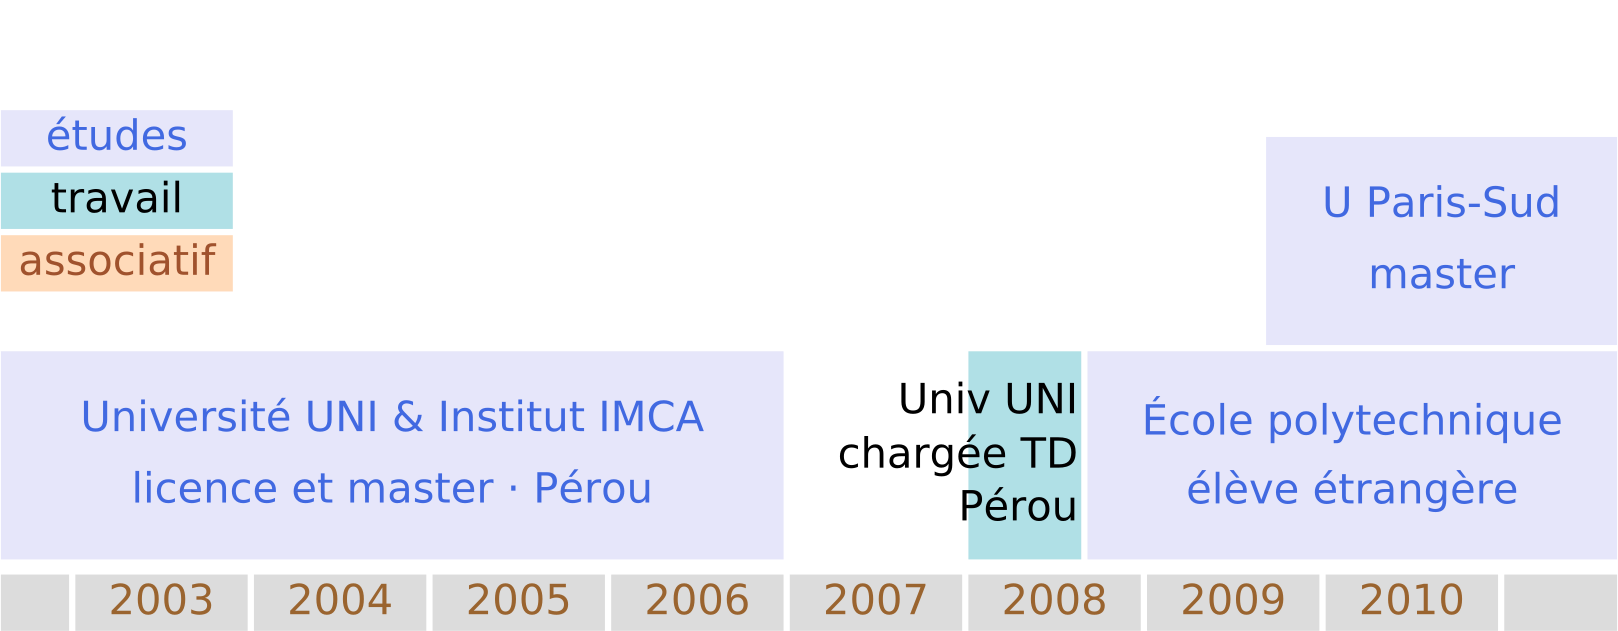
\includegraphics[width=0.9\textwidth,height=\textheight]{img/alba-timeline-etudes.png}

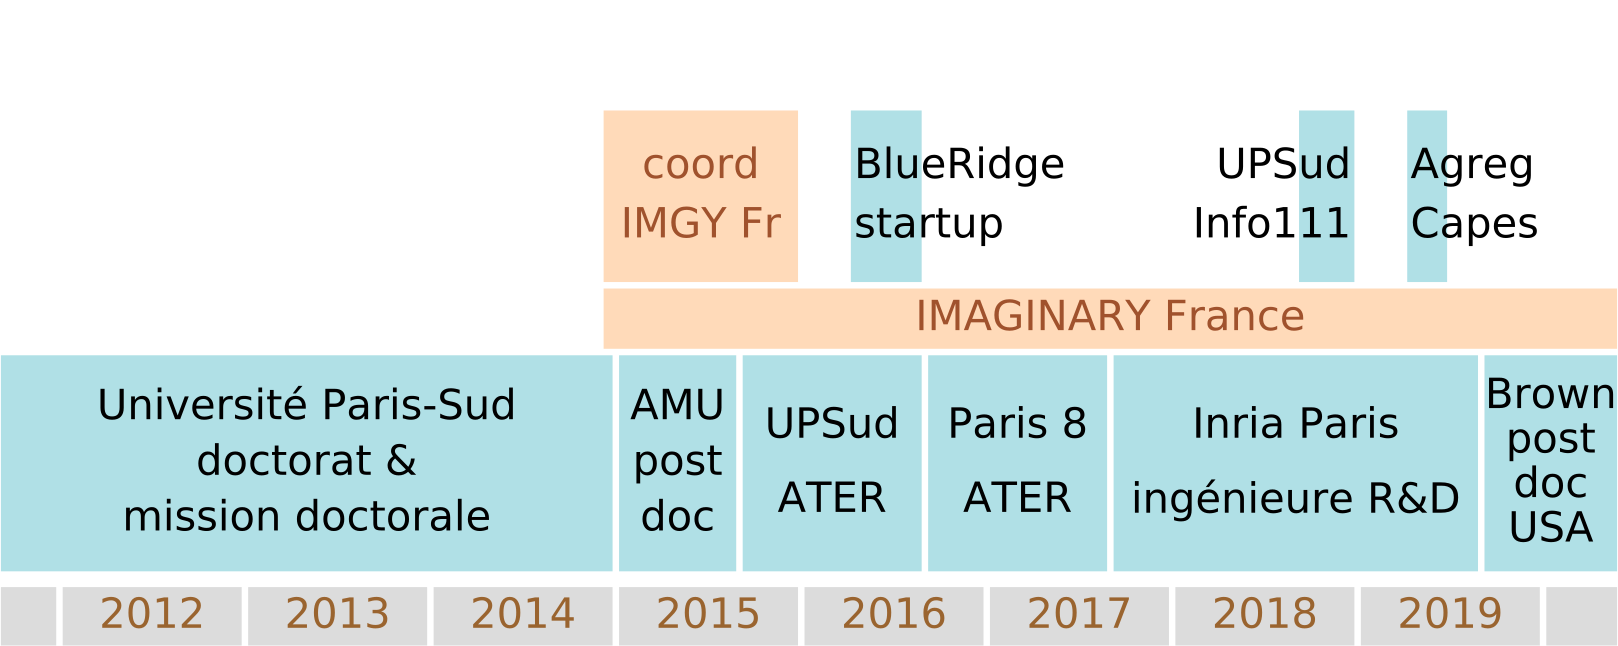
\includegraphics[width=0.9\textwidth,height=\textheight]{img/alba-timeline-viepro.png}
\end{frame}

\begin{frame}{Systèmes dynamiques}
\protect\hypertarget{systuxe8mes-dynamiques}{}
\begin{itemize}
\tightlist
\item
  Billards - cylindres discrets
\end{itemize}

\smallskip

\centering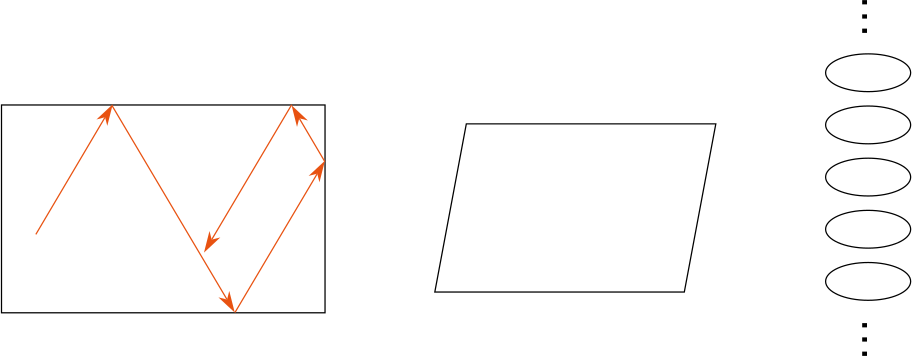
\includegraphics[width=\textwidth,height=0.25\textheight]{img/billard-cylindre.png}

\par

\smallskip

\begin{itemize}
\tightlist
\item
  La saga des escaliers et des wind-trees
\end{itemize}

\smallskip

\centering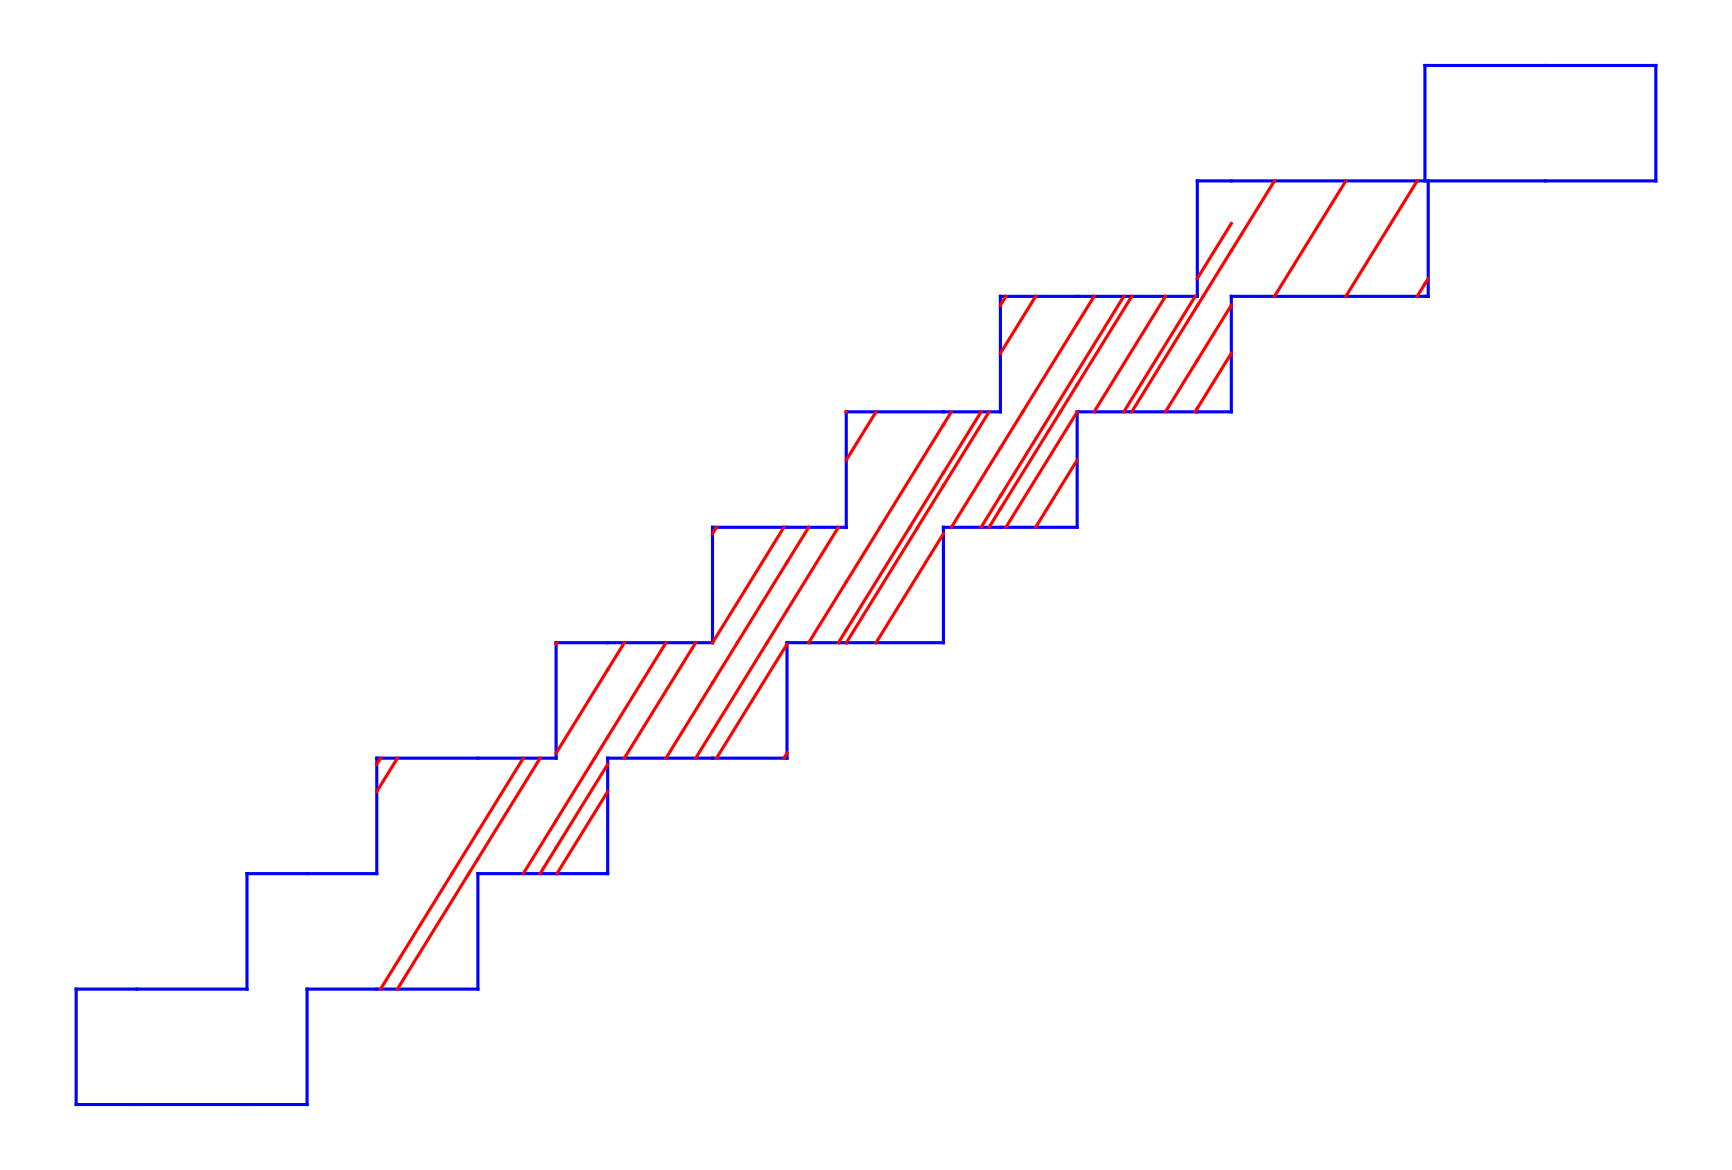
\includegraphics[width=\textwidth,height=0.25\textheight]{img/escalier-recollement-variable.png}\qquad
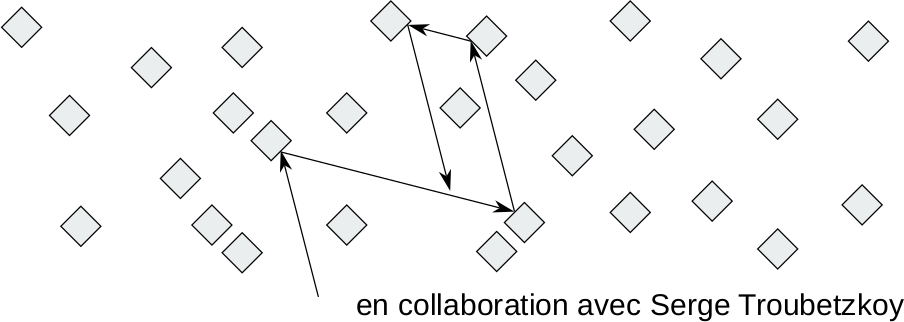
\includegraphics[width=\textwidth,height=0.25\textheight]{img/wind-tree.png}

\par
\end{frame}

\begin{frame}{Ma thèse}
\protect\hypertarget{ma-thuxe8se}{}
Thèse soutenue en 2014 à Orsay:

\emph{Étude d'une famille de transformations\\
préservant la mesure de \(ℤ × 𝕋\).}

sous la direction de Jean-Christophe Yoccoz (Collège de France).

Résultats sur \(ℤ × 𝕋\) \(\longleftrightarrow\) escaliers infinis.

\textbf{Thm} (2014) Direction fixée, escalier générique:\\
dynamique conservative, minimale et ergodique.
\end{frame}

\begin{frame}{Mes travaux avec Serge Troubetzkoy}
\protect\hypertarget{mes-travaux-avec-serge-troubetzkoy}{}
Des résultats de plus en plus précis.

\textbf{Thm} (2015) Génériquement, la dynamique du wind-tree est
minimale dans un large ensemble de directions.

\textbf{Thm} (2016) Génériquement, la dynamique du wind-tree dans
presque toute direction est ergodique.

\textbf{Thm} (2016) La dynamique d'un billard VH est faiblement
mélangeante dans un large ensemble de directions.

\textbf{Thm} (2017) Génériquement, la dynamique du wind-tree est
d'indice ergodique infini dans un large ensemble de directions.

\textbf{Thm} (2019) Génériquement, la dynamique des surfaces en escalier
est uniquement ergodique dans un large ensemble de directions.

\textbf{Thm} (2019) Génériquement, la dynamique du wind-tree est
uniquement ergodique dans un large ensemble de directions.
\end{frame}

\begin{frame}{Génération de maillages 1}
\protect\hypertarget{guxe9nuxe9ration-de-maillages-1}{}
\begin{block}{Reproduction d'objets mathématiques}
\protect\hypertarget{reproduction-dobjets-mathuxe9matiques}{}
\begin{description}
\tightlist
\item[Contexte]
Diffusion auprès du grand public
\end{description}

\smallskip\centering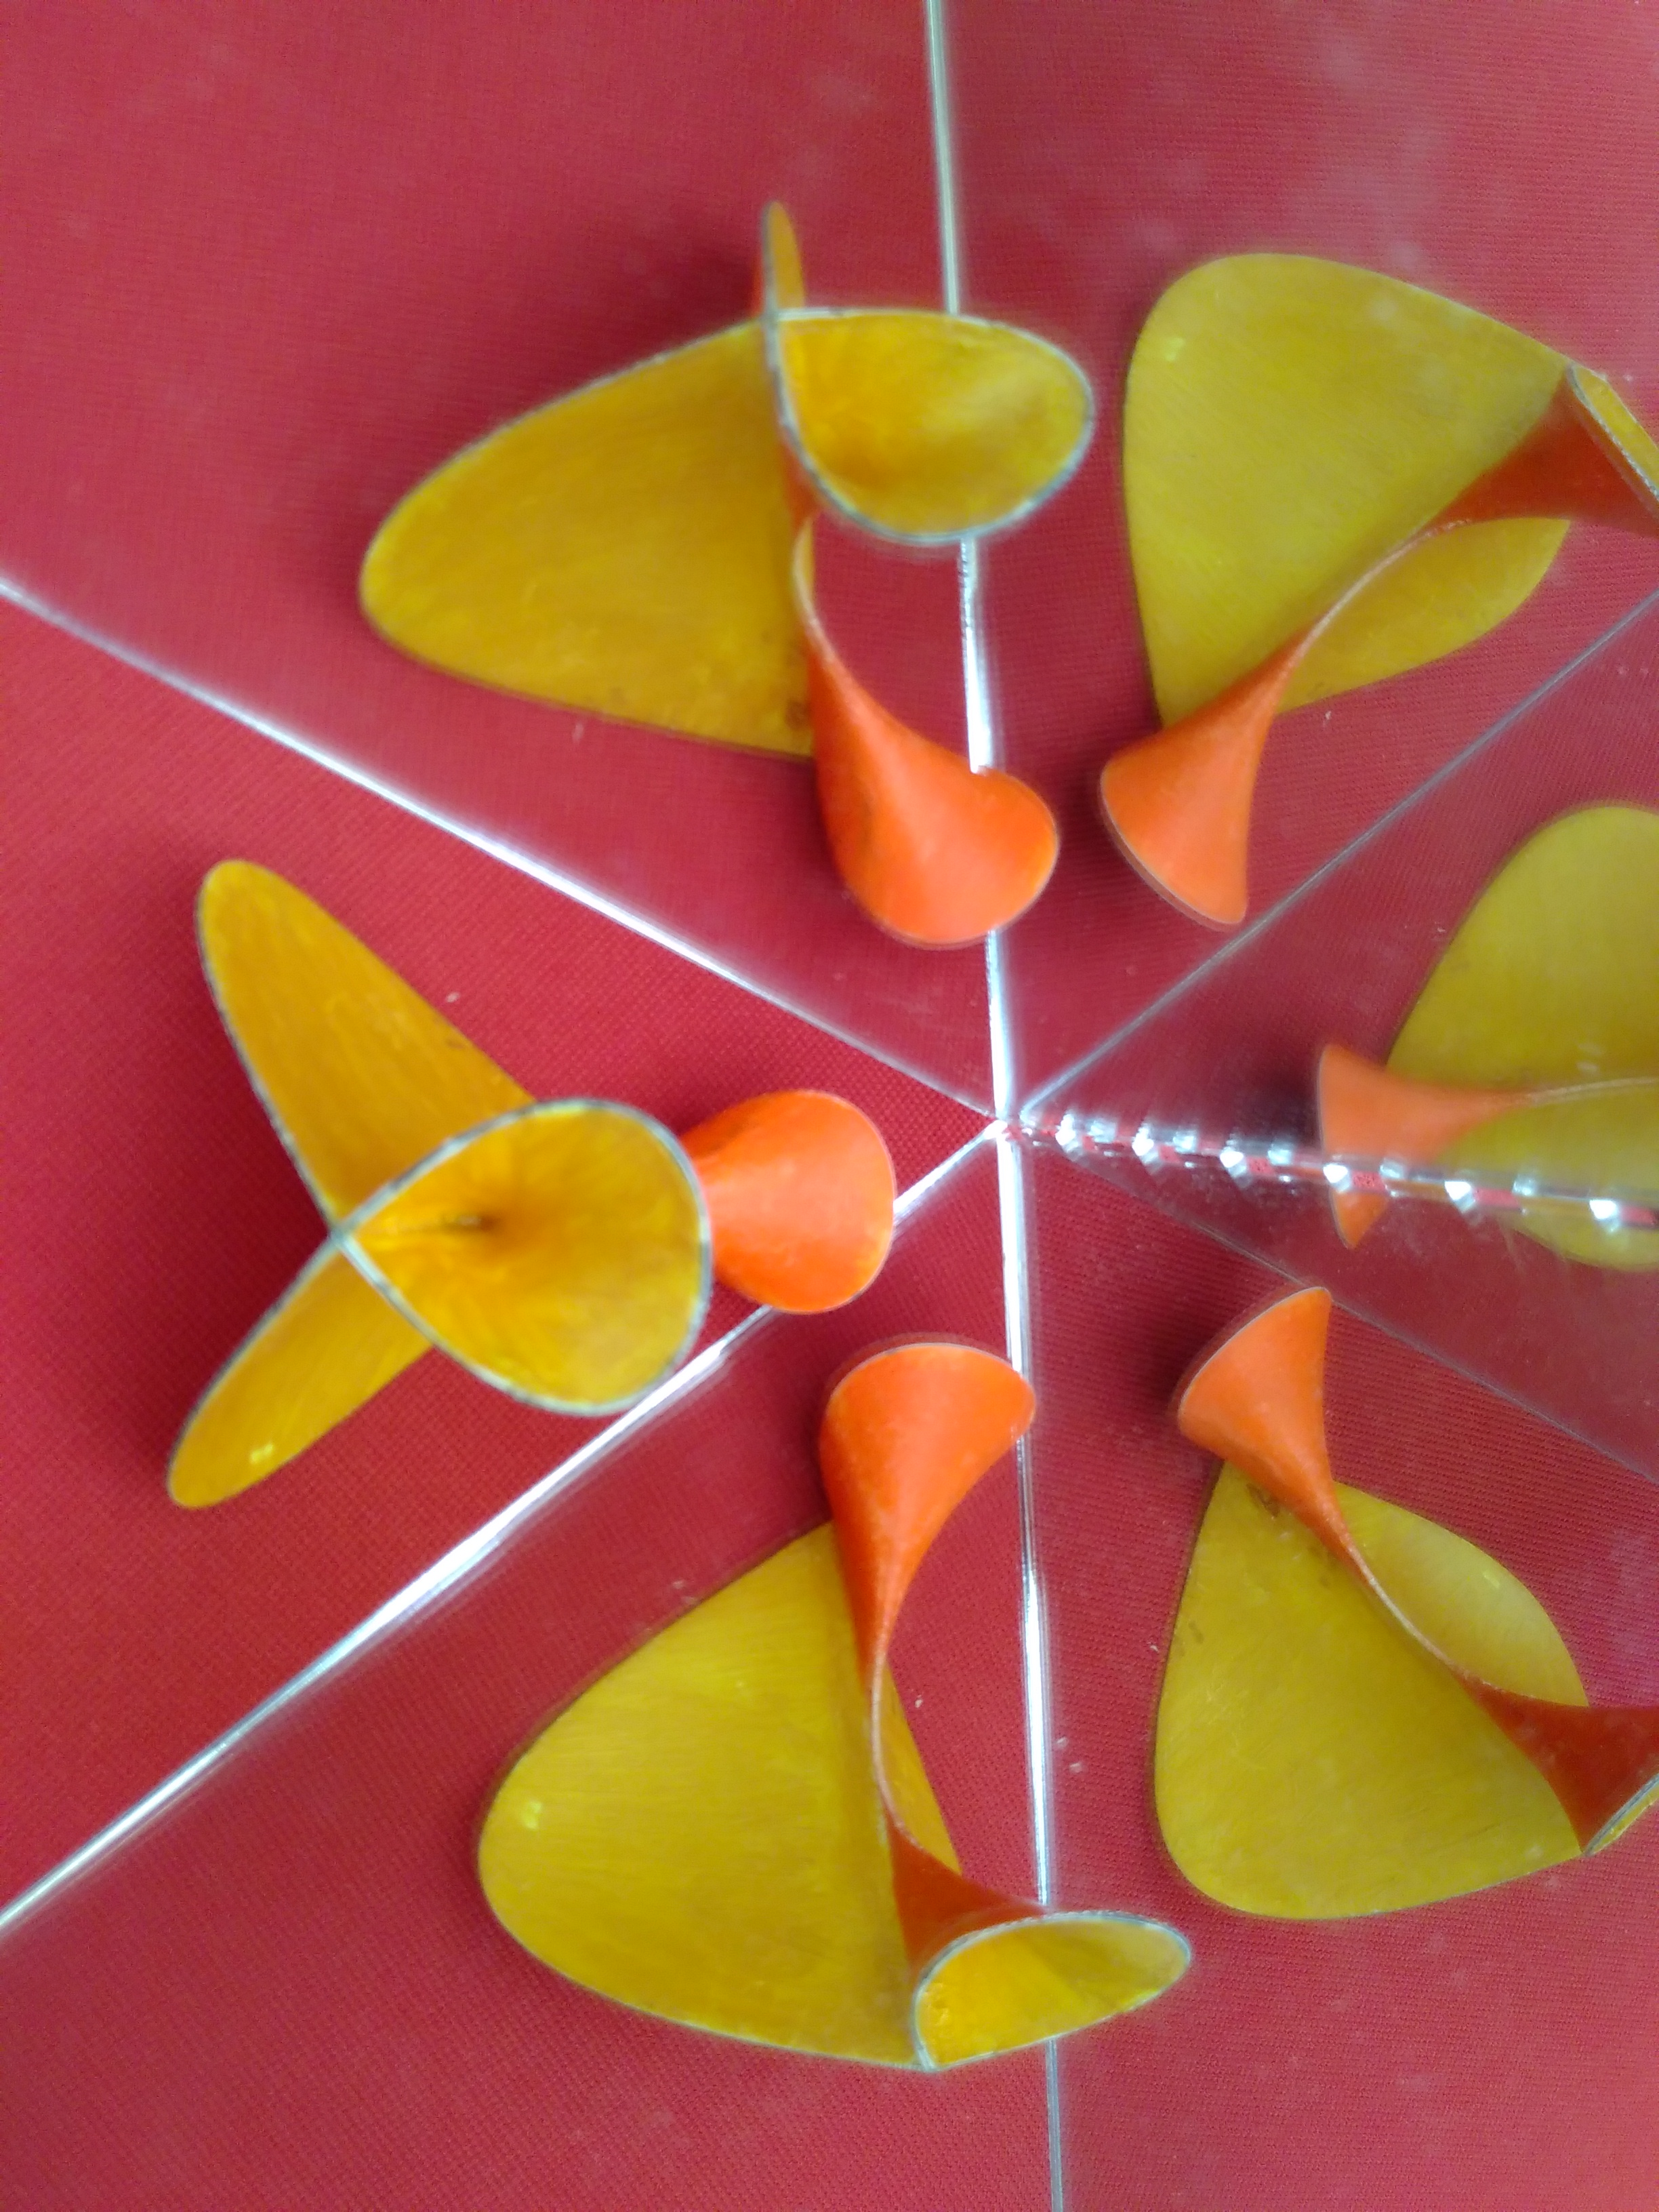
\includegraphics[width=\textwidth,height=0.25\textheight]{img/3D-Kolibri-bicolore.jpg}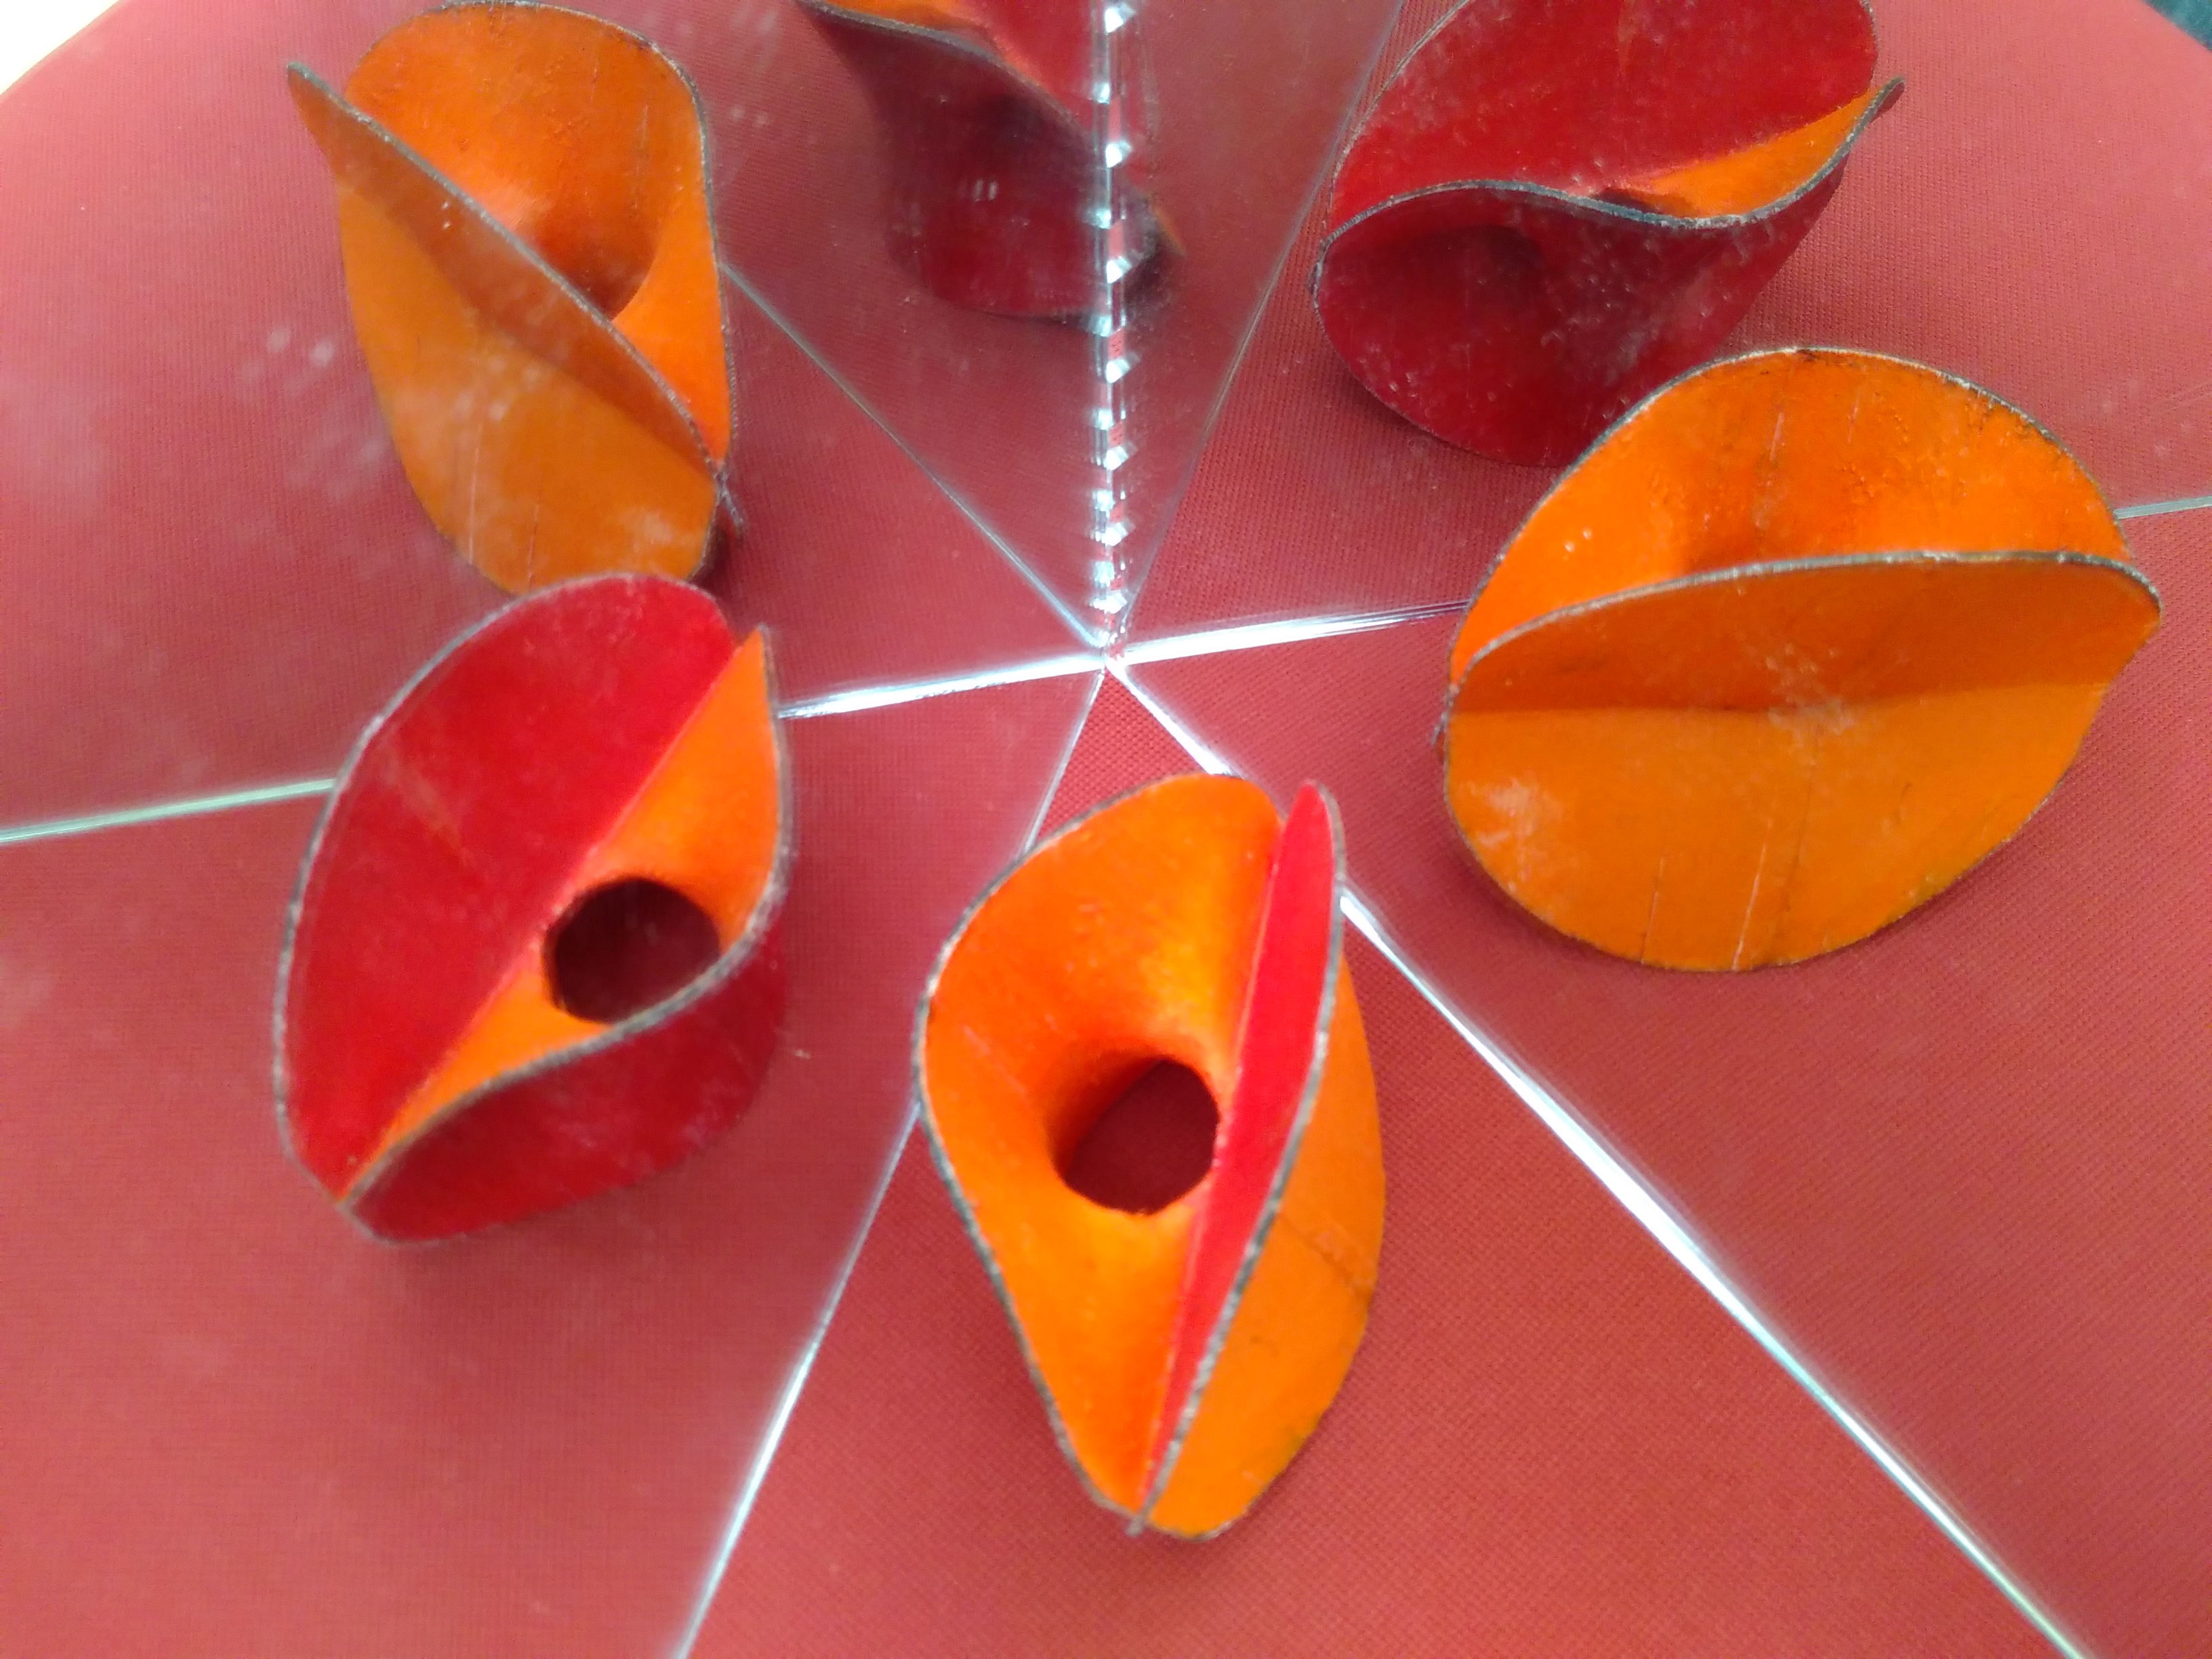
\includegraphics[width=\textwidth,height=0.25\textheight]{img/3D-Herz-colorie.jpg}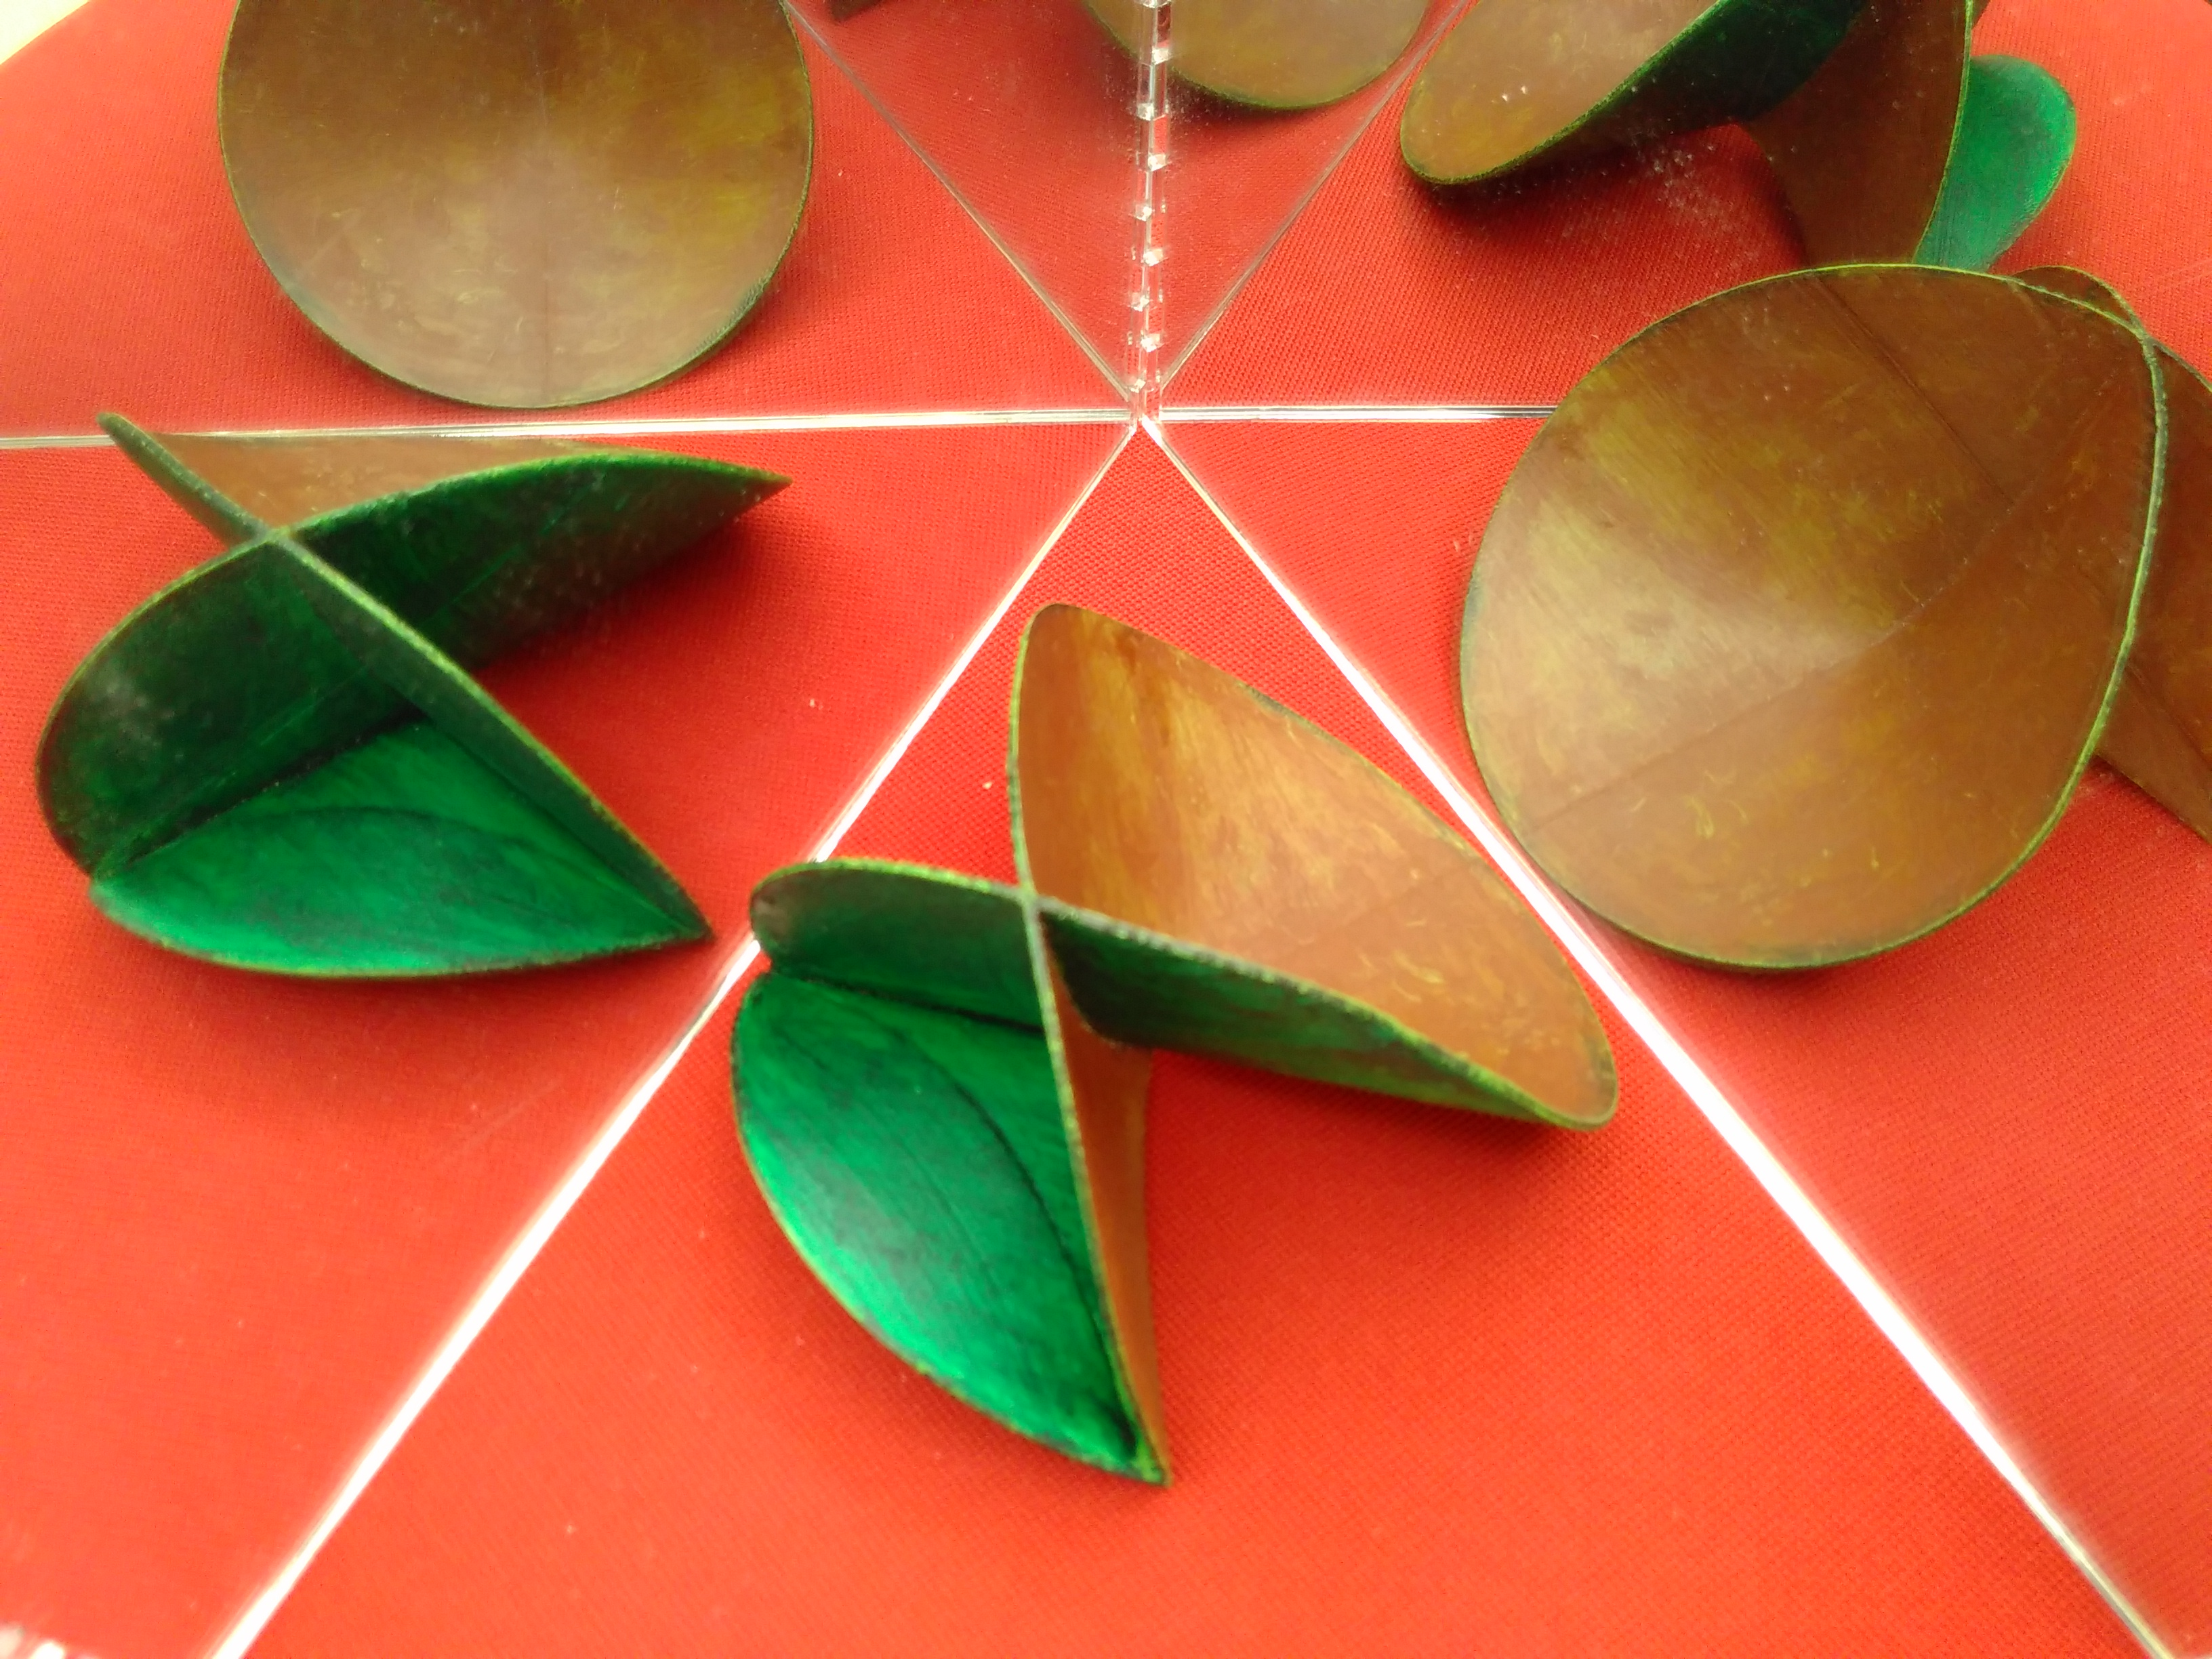
\includegraphics[width=\textwidth,height=0.25\textheight]{img/3D-Taube-coloriee.jpg}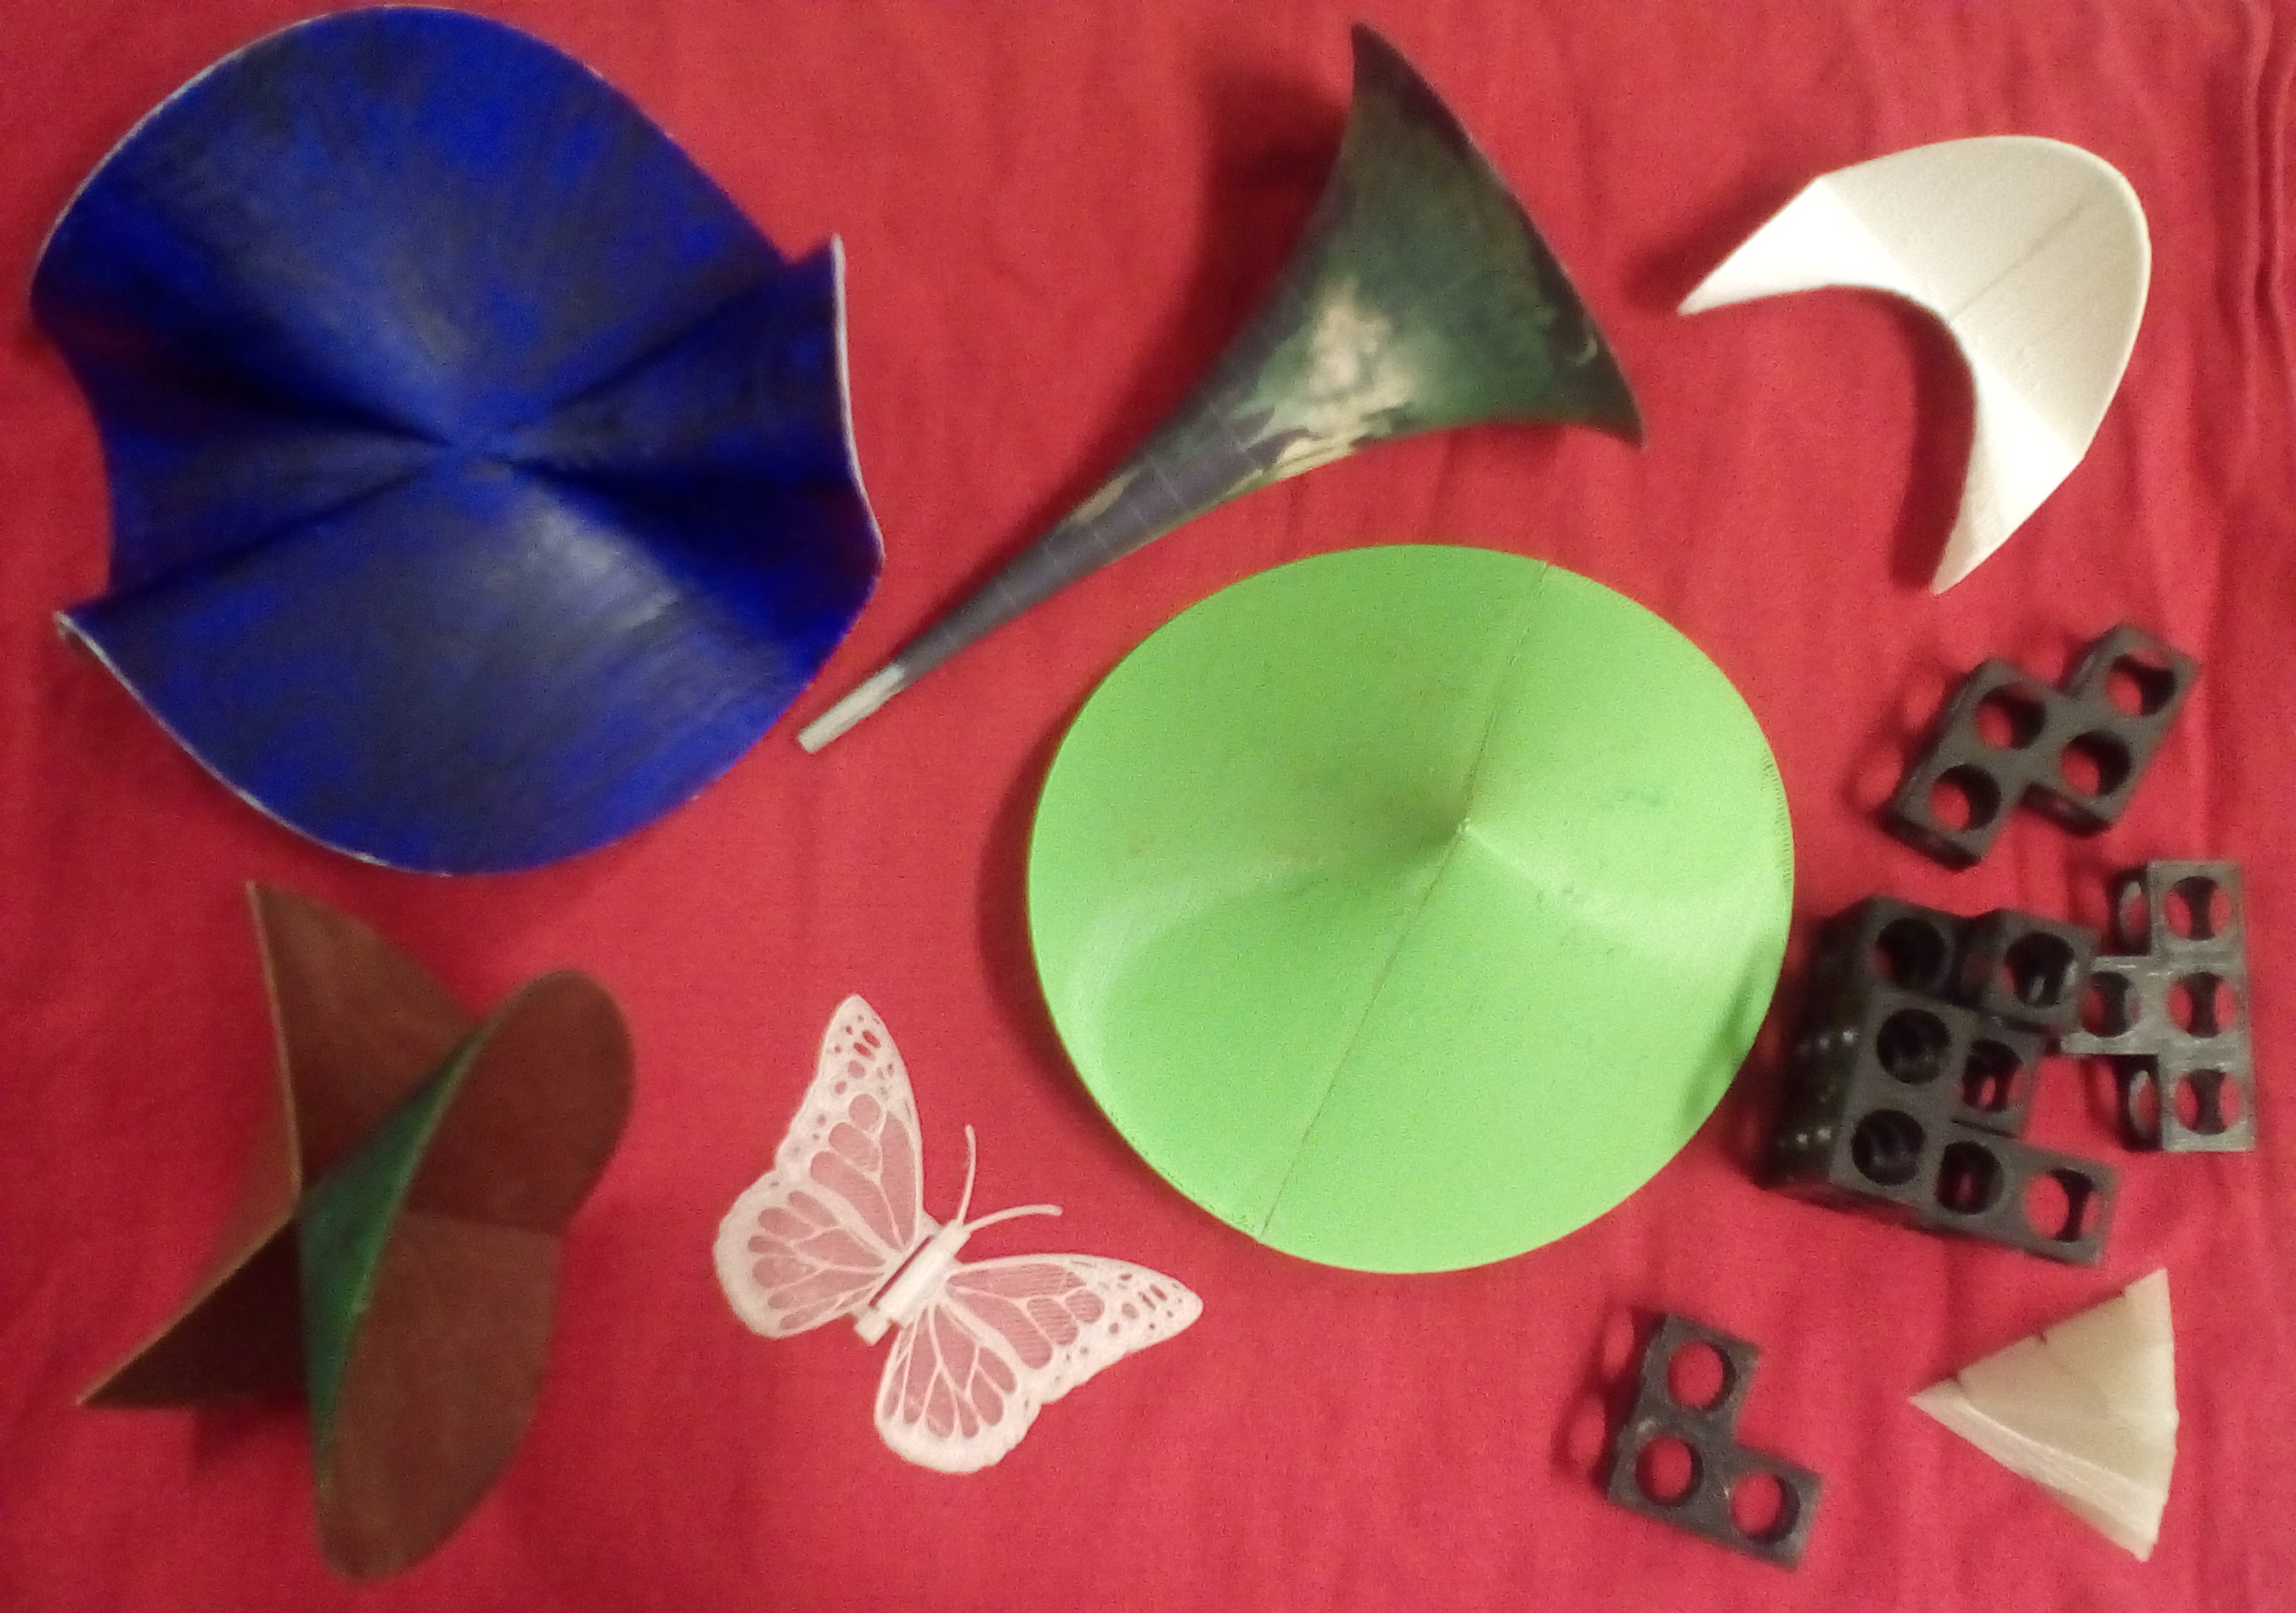
\includegraphics[width=\textwidth,height=0.25\textheight]{img/objets-3D-sur-echarpe-rouge.png}

\par\smallskip

\begin{description}
\tightlist
\item[But]
Des méthodes pour automatiser ou semi-automatiser la production de
larges catégories d'objets : surfaces algébriques, surfaces minimales,
objets fractals, arbres, pavages, \emph{\ldots{} mais aussi reproduction
d'objets historiques.}
\end{description}
\end{block}
\end{frame}

\begin{frame}{Génération de maillages 2}
\protect\hypertarget{guxe9nuxe9ration-de-maillages-2}{}
\begin{block}{Adaptation de formes - le problème du zoom}
\protect\hypertarget{adaptation-de-formes---le-probluxe8me-du-zoom}{}
\begin{description}
\tightlist
\item[Contexte]
Nombreux objets de musées numérisés en 3D.
\item[Problème]
Les représenter beaucoup plus grands que nature.
\end{description}

\smallskip\centering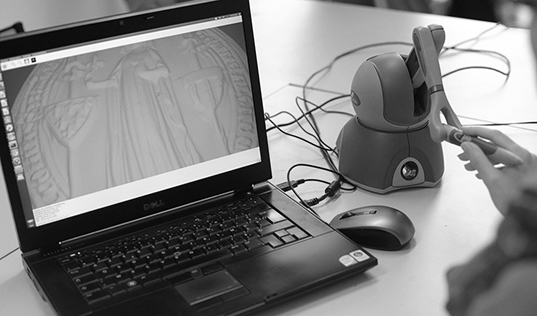
\includegraphics[width=\textwidth,height=0.6\textheight]{img/bras-haptique.jpg}

\par\smallskip

\begin{description}
\tightlist
\item[Idée]
Raffiner le maillage\\
\emph{en s'adaptant à l'exploration de l'utilisateur}.
\end{description}
\end{block}
\end{frame}

\begin{frame}{Génération de maillages 3}
\protect\hypertarget{guxe9nuxe9ration-de-maillages-3}{}
\begin{block}{Adaptation de formes - projection sur des surfaces}
\protect\hypertarget{adaptation-de-formes---projection-sur-des-surfaces}{}
\begin{description}
\tightlist
\item[Contexte]
On veut projeter une image ou une vidéo.
\item[Problème]
La surface de projection ne correspond pas\\
à la surface ``naturelle'' de la vidéo.

\strut
\end{description}

\smallskip\centering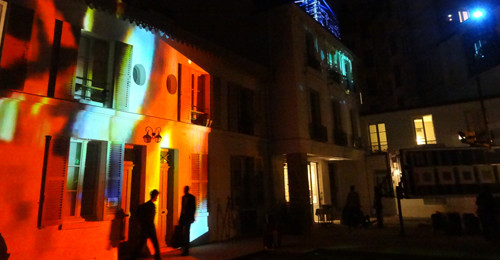
\includegraphics[width=\textwidth,height=0.5\textheight]{img/Neticlab-Paysage-500x260.jpg}

\par\smallskip

\begin{description}
\tightlist
\item[Idée]
Déformer le maillage\\
\emph{en s'adaptant au contexte de l'utilisateur}.
\end{description}
\end{block}
\end{frame}

\begin{frame}{Analyse de nuages de points}
\protect\hypertarget{analyse-de-nuages-de-points}{}
\begin{block}{À la recherche des équations perdues}
\protect\hypertarget{uxe0-la-recherche-des-uxe9quations-perdues}{}
\begin{description}
\tightlist
\item[Contexte]
Objets illustrant des idées mathématiques.
\item[Problème]
Description incomplète.
\item[But]
Compléter la description pour reproduire l'objet.
\end{description}

\smallskip\centering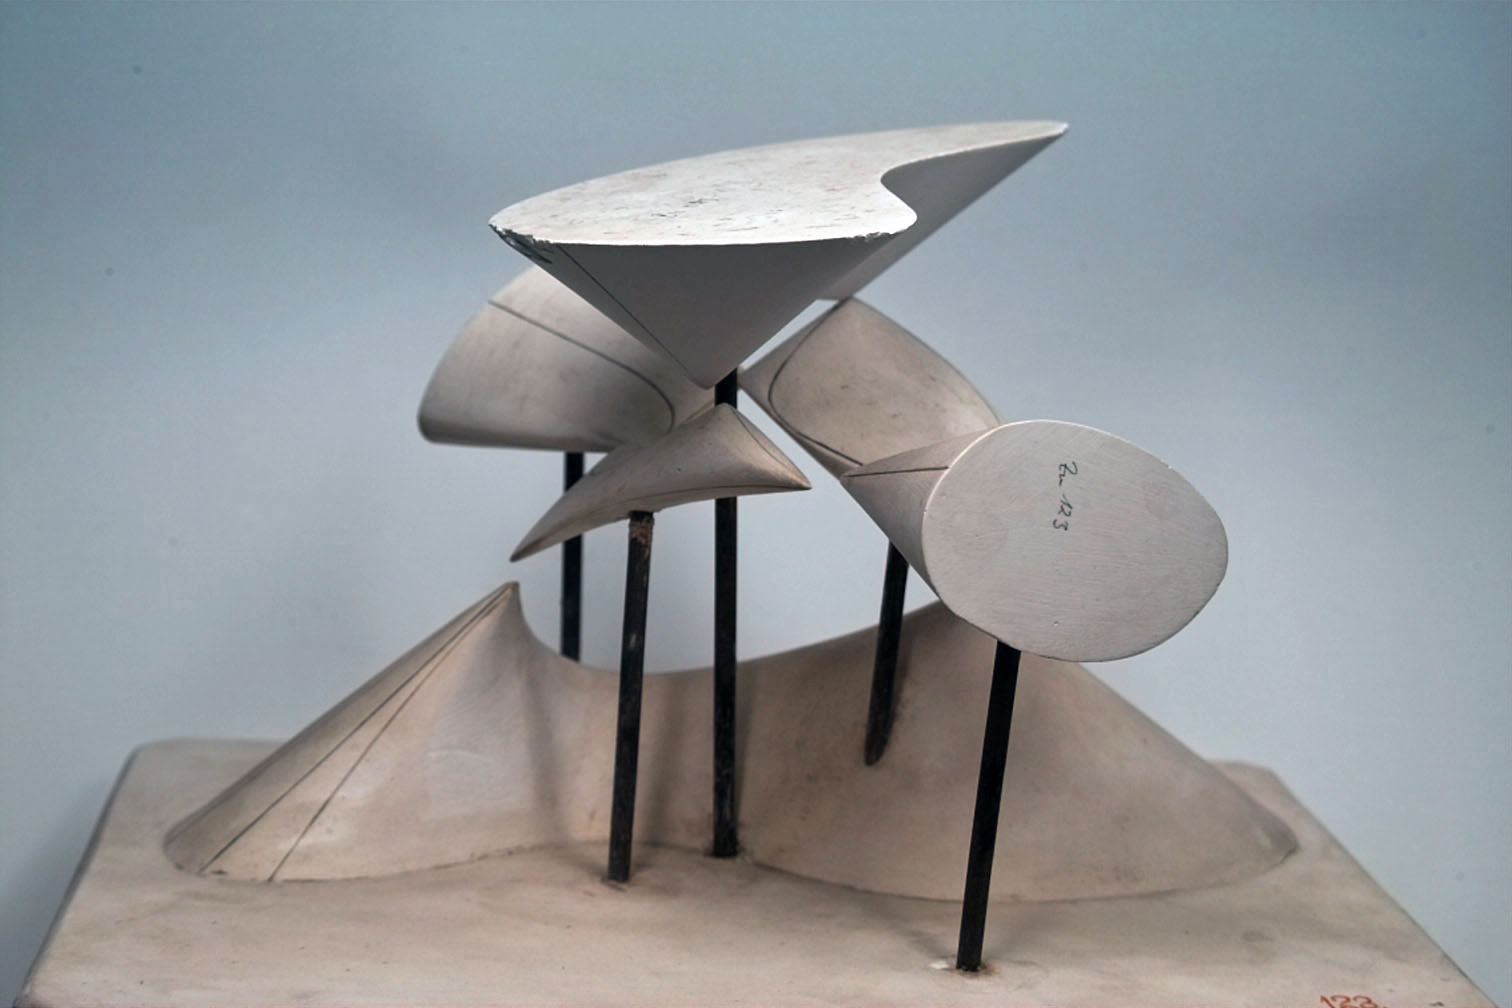
\includegraphics[width=\textwidth,height=0.25\textheight]{img/kummer-photo.jpg}

\includegraphics[width=\textwidth,height=0.25\textheight]{img/kummer-surfer.png}
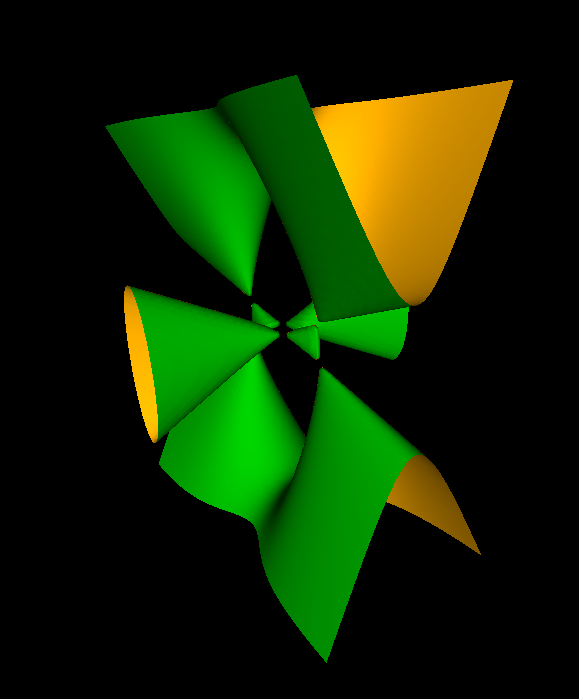
\includegraphics[width=\textwidth,height=0.25\textheight]{img/kummer-mathmod.png}
\({}\) \({}\) \({}\) ???

\par\smallskip

\begin{description}
\tightlist
\item[Idée]
Numériser puis analyser.
\end{description}
\end{block}
\end{frame}

\begin{frame}{Réparation de maillages}
\protect\hypertarget{ruxe9paration-de-maillages}{}
\begin{block}{Subtilités de la fabrication additive}
\protect\hypertarget{subtilituxe9s-de-la-fabrication-additive}{}
\begin{description}
\tightlist
\item[Contexte]
Imprimer un objet 3D de source externe.
\item[Problème]
Maillage défectueux.
\item[But]
Réparer le fichier pour une impression de qualité.
\end{description}

\smallskip\centering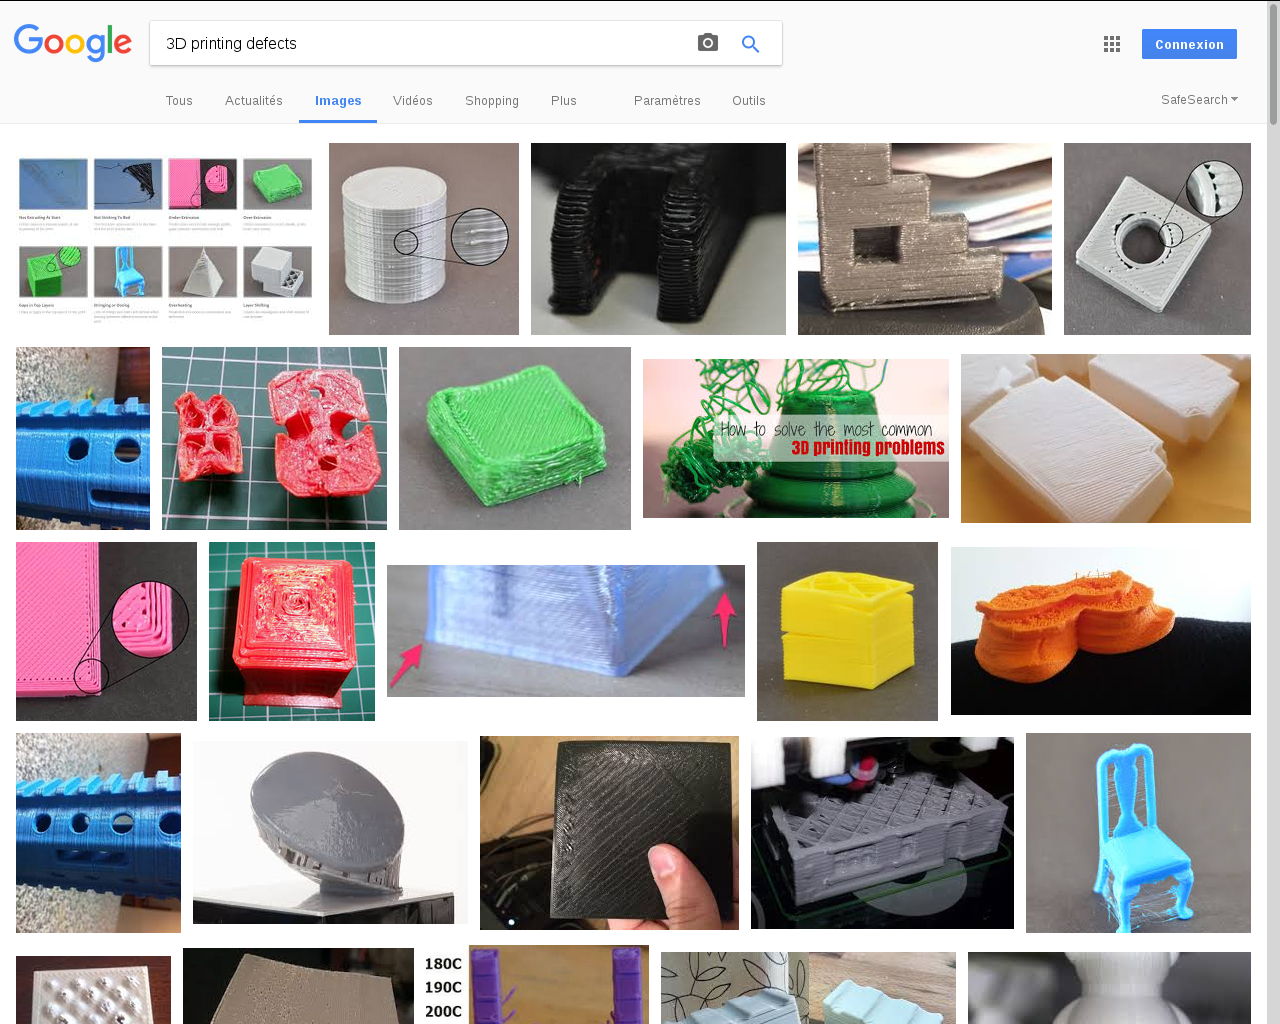
\includegraphics[width=\textwidth,height=0.6\textheight]{img/screenshot-google-3d-printing-defects.png}

\par\smallskip
\end{block}
\end{frame}

\begin{frame}{Maillages volumiques}
\protect\hypertarget{maillages-volumiques}{}
\begin{block}{Polyèdres à surface minimale}
\protect\hypertarget{polyuxe8dres-uxe0-surface-minimale}{}
\begin{description}
\tightlist
\item[Question]
Quelle configuration de \(n\) points dans l'espace minimise la surface
de leur enveloppe convexe à volume fixé?
\item[Réponse]
Akiyama donne la réponse pour \(n=4\) à \(12\) en 2017.
\end{description}

\smallskip\centering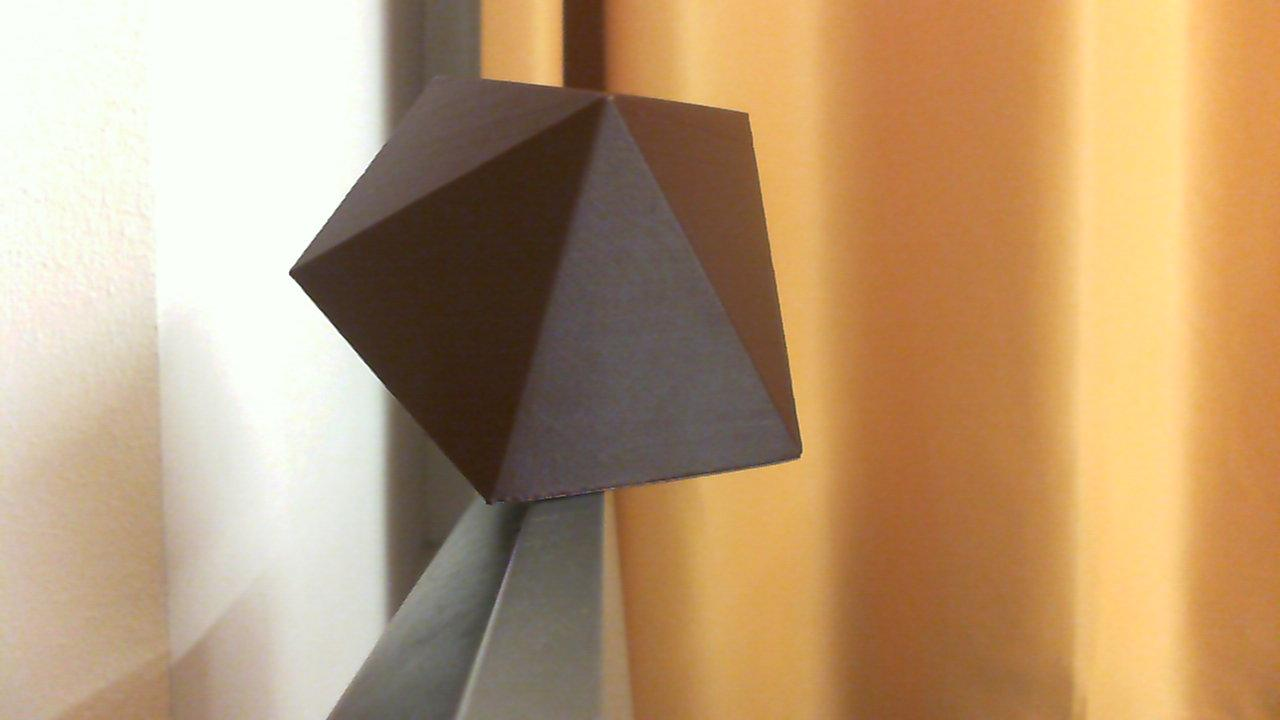
\includegraphics[width=\textwidth,height=0.25\textheight]{img/akiyama8hull3dprint-1.jpg}

\par\smallskip

\begin{description}
\tightlist
\item[Questions]
Que se passe-t-il pour \(n\) grand? Y a-t-il des formes de faces qui se
repètent? Peut-on paver l'espace avec ce type de polyèdres?
\end{description}
\end{block}
\end{frame}

\begin{frame}{Expérience d'enseignement}
\protect\hypertarget{expuxe9rience-denseignement}{}
\textbf{\textgreater600h} dont 192h responsable de cours

\begin{longtable}[]{@{}llll@{}}
\toprule
\endhead
2016-2017 & U Paris 8 (192h) & info &

\includegraphics[width=\textwidth,height=0.05\textheight]{img/logo-up8.png}\tabularnewline
2015-2016 & U Paris-Sud (192h) & math &

\includegraphics[width=\textwidth,height=0.05\textheight]{img/logo-upsaclay.png}\tabularnewline
2014 & U Paris-Sud (96h) & math &

\includegraphics[width=\textwidth,height=0.05\textheight]{img/logo-upsud.png}\tabularnewline
2008 & UNI (192h) & math &

\includegraphics[width=\textwidth,height=0.05\textheight]{img/logo-uni.png}\tabularnewline
\bottomrule
\end{longtable}
\end{frame}

\begin{frame}{Cours, cours intégrés, TD}
\protect\hypertarget{cours-cours-intuxe9gruxe9s-td}{}
J'ai enseigné

\begin{itemize}
\tightlist
\item
  Équations différentielles
\item
  Mathématiques numériques avec Python
\item
  Calculus
\item
  Analyse
\item
  Calcul formel avec SageMath
\item
  Structures algébriques
\item
  Gestion de contenu avec Wordpress
\item
  Algèbre linéaire
\item
  Calcul vectoriel
\item
  Calcul intégral
\item
  Programmation orientée objet avec Java
\end{itemize}
\end{frame}

\begin{frame}{Adaptation à l'enseignement de l'UTT}
\protect\hypertarget{adaptation-uxe0-lenseignement-de-lutt}{}
Alternance

\begin{itemize}
\tightlist
\item
  j'ai déjà encadré un étudiant géomaticien de Paris 8\\
  en alternance à l'Établissement français du sang
\item
  j'ai déjà enseigné deux cours en utilisant CoCalc,\\
  plateforme collaborative en ligne qui se prête bien\\
  à la pédagogie inversée
\end{itemize}

UEs LO13 ``Infographie 3D : théorie et applications''

\begin{itemize}
\tightlist
\item
  passion de l'impression 3D
\item
  curiosité vis-à-vis de la réalité virtuelle
\end{itemize}

Respect de l'apprenant
\end{frame}

\begin{frame}{Proposition de projet tutoré}
\protect\hypertarget{proposition-de-projet-tutoruxe9}{}
\begin{longtable}[]{@{}lcr@{}}
\toprule
\endhead
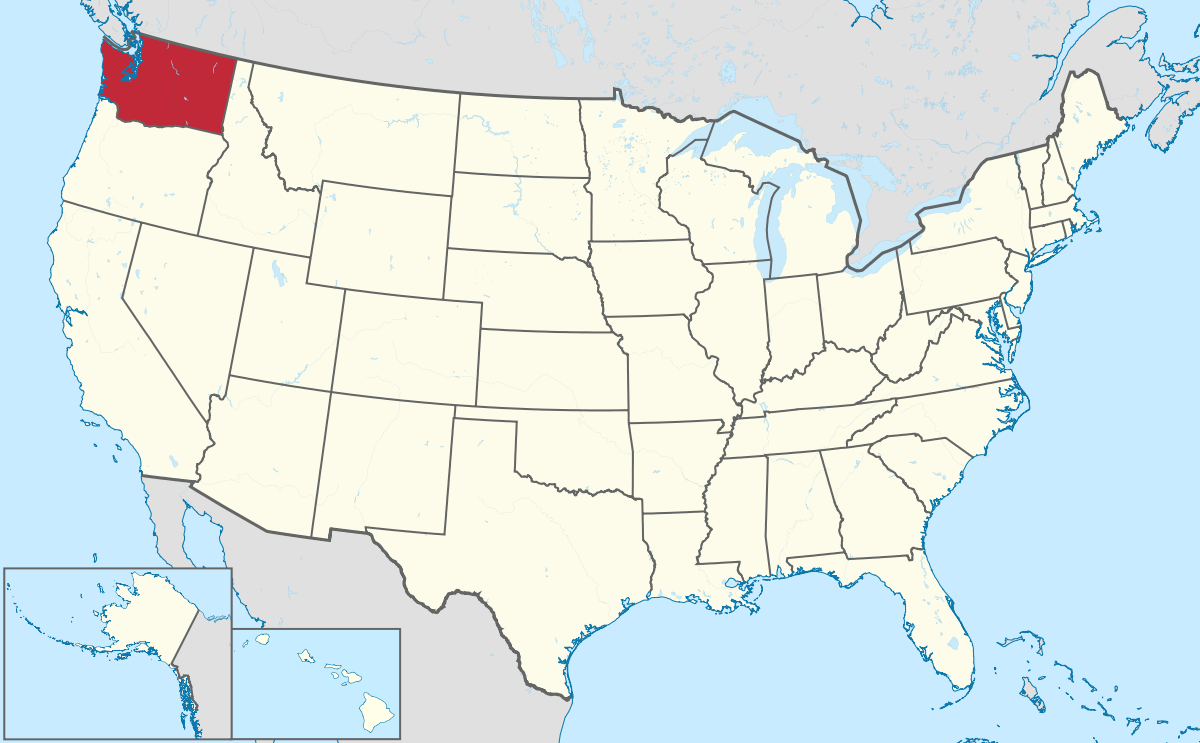
\includegraphics[width=\textwidth,height=0.25\textheight]{img/USARed.png}
& \(\longleftrightarrow\) &
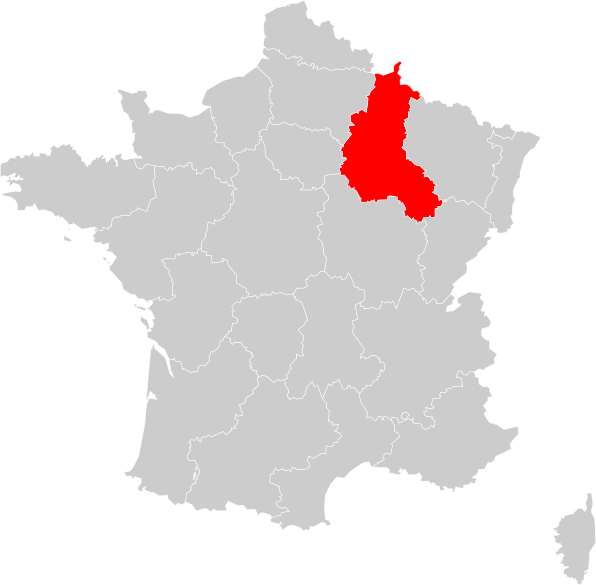
\includegraphics[width=\textwidth,height=0.25\textheight]{img/FranceRed.png}\tabularnewline
U. Washington & & UTT\tabularnewline
3-4 students & & 3-4 étudiants\tabularnewline
J. Athreya & & A. Málaga\tabularnewline
\bottomrule
\end{longtable}
\end{frame}

\begin{frame}{Expérience en entreprise}
\protect\hypertarget{expuxe9rience-en-entreprise}{}
\begin{itemize}
\tightlist
\item
  Stage de 2e année à La Défense, 2012
\end{itemize}

\centering 
\includegraphics[width=\textwidth,height=0.1\textheight]{img/logo-sechilienne.png}

\par

\begin{itemize}
\tightlist
\item
  Développeuse freelance chez BlueRidge Logiciels, 2016
\end{itemize}

\centering 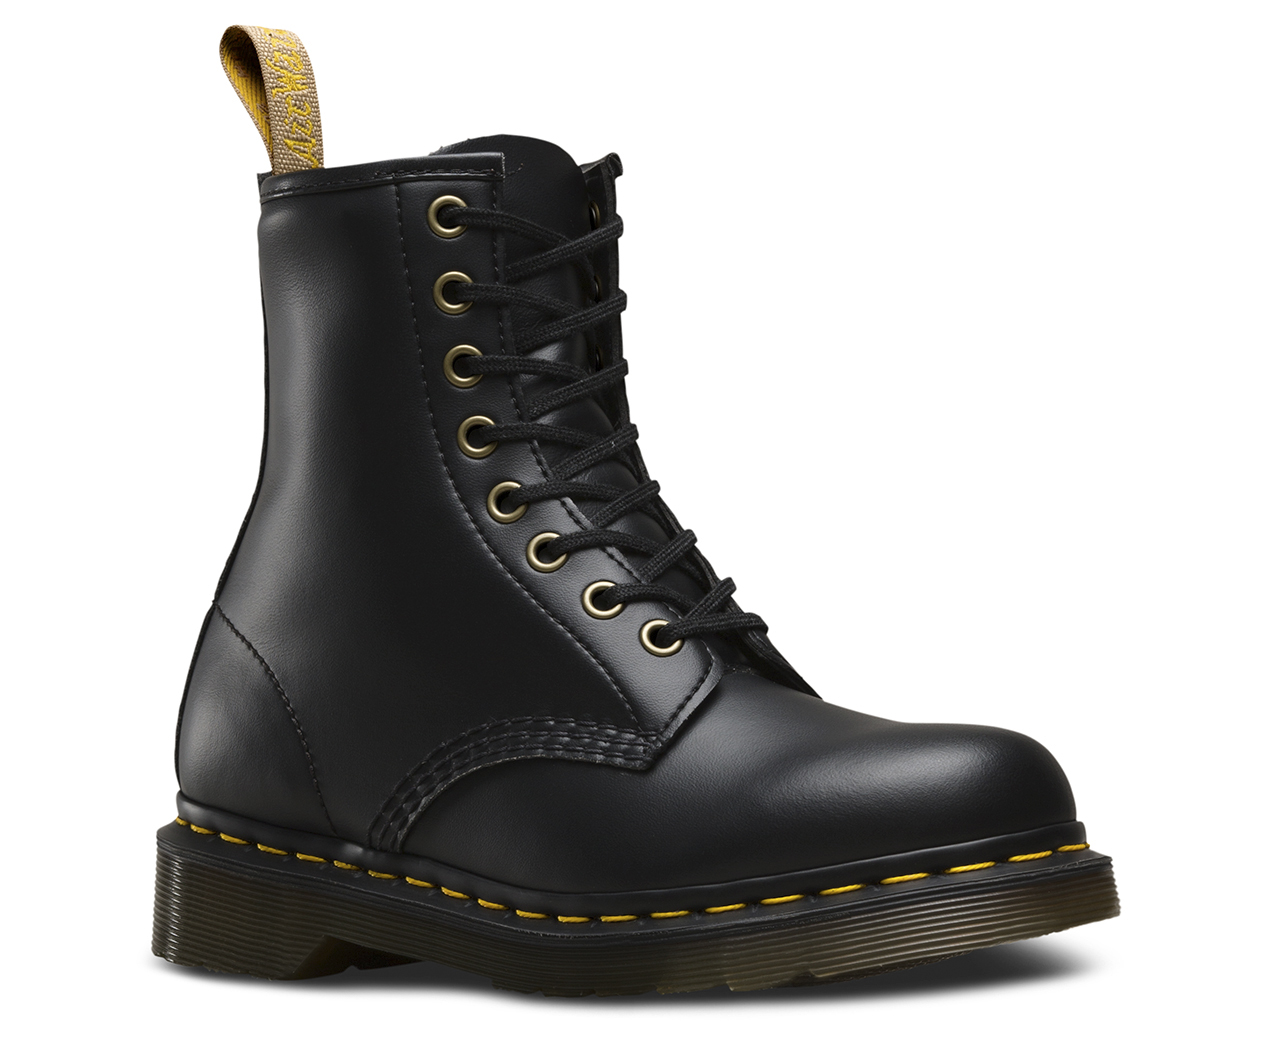
\includegraphics[width=\textwidth,height=0.2\textheight]{img/botte.jpg}

\par
\end{frame}

\begin{frame}{Networking/réseau}
\protect\hypertarget{networkingruxe9seau}{}
Environnements startups / université / makers

\begin{longtable}[]{@{}lll@{}}
\toprule
Tiers-lieux & Fabrication numérique & Meetups\tabularnewline
\midrule
\endhead
Réso-nance & LFO & Ladies of code\tabularnewline
Proto204 & Small Lab & Le Wagon\tabularnewline
e-sas & Fablab Digiscope & Wolfox\tabularnewline
& X-F4B & \ldots{}\tabularnewline
& Carrefour numérique &\tabularnewline
& \ldots{} &\tabularnewline
\bottomrule
\end{longtable}
\end{frame}

\begin{frame}{Responsabilités administratives}
\protect\hypertarget{responsabilituxe9s-administratives}{}
\begin{itemize}
\item
  Faire vivre le département

  \begin{itemize}
  \tightlist
  \item
    stages
  \item
    projets tutorés
  \item
    emplois du temps
  \item
    forums
  \item
    admissions
  \item
    portes ouvertes
  \end{itemize}
\end{itemize}

\centering 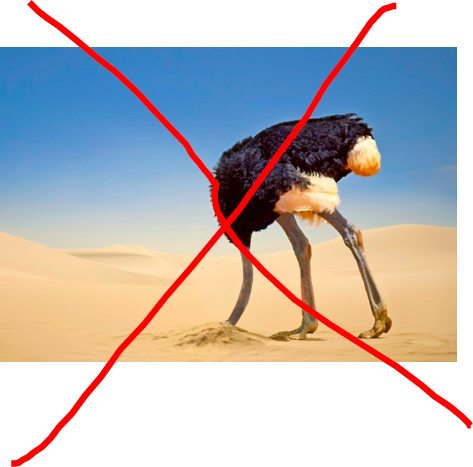
\includegraphics[width=\textwidth,height=0.25\textheight]{img/pas-autruche.png}

\par

\begin{itemize}
\item
  Actions de sensibilisation

  \begin{itemize}
  \tightlist
  \item
    fête de la Science
  \item
    nuit des chercheurs
  \end{itemize}
\end{itemize}
\end{frame}

\begin{frame}{La médiation scientifique}
\protect\hypertarget{la-muxe9diation-scientifique}{}
\begin{itemize}
\tightlist
\item
  médiation autour de projets art-science -- « La lumière ne s'arrête
  pas là » -- « Premières intimités de l'être » -- « Turbulent »
\end{itemize}

\centering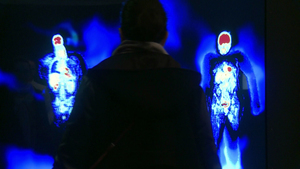
\includegraphics[width=\textwidth,height=0.15\textheight]{img/premiere-intimite-de-letre.jpg}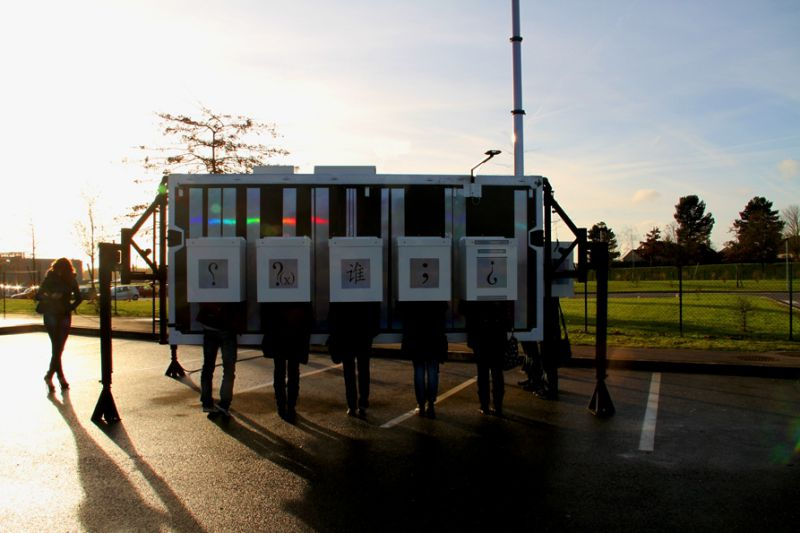
\includegraphics[width=\textwidth,height=0.15\textheight]{img/chambre-de-lorentz.jpg}

\par

\begin{itemize}
\tightlist
\item
  IMAGINARY France -- plus de 100 heures face au grand public -- 10
  événements organisés ; une rencontre autour des plateformes de partage
  -- résautage actif : incitation à de nouvelles contributions, gestion
  des bénévoles
\end{itemize}

\centering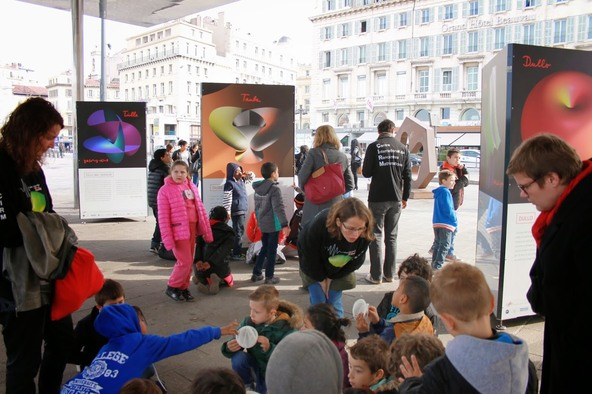
\includegraphics[width=\textwidth,height=0.25\textheight]{img/vieux-port-alba.jpg}

\par
\end{frame}

\begin{frame}{La recherche de fonds}
\protect\hypertarget{la-recherche-de-fonds}{}
\begin{block}{Blocage et illumination}
\protect\hypertarget{blocage-et-illumination}{}
\centering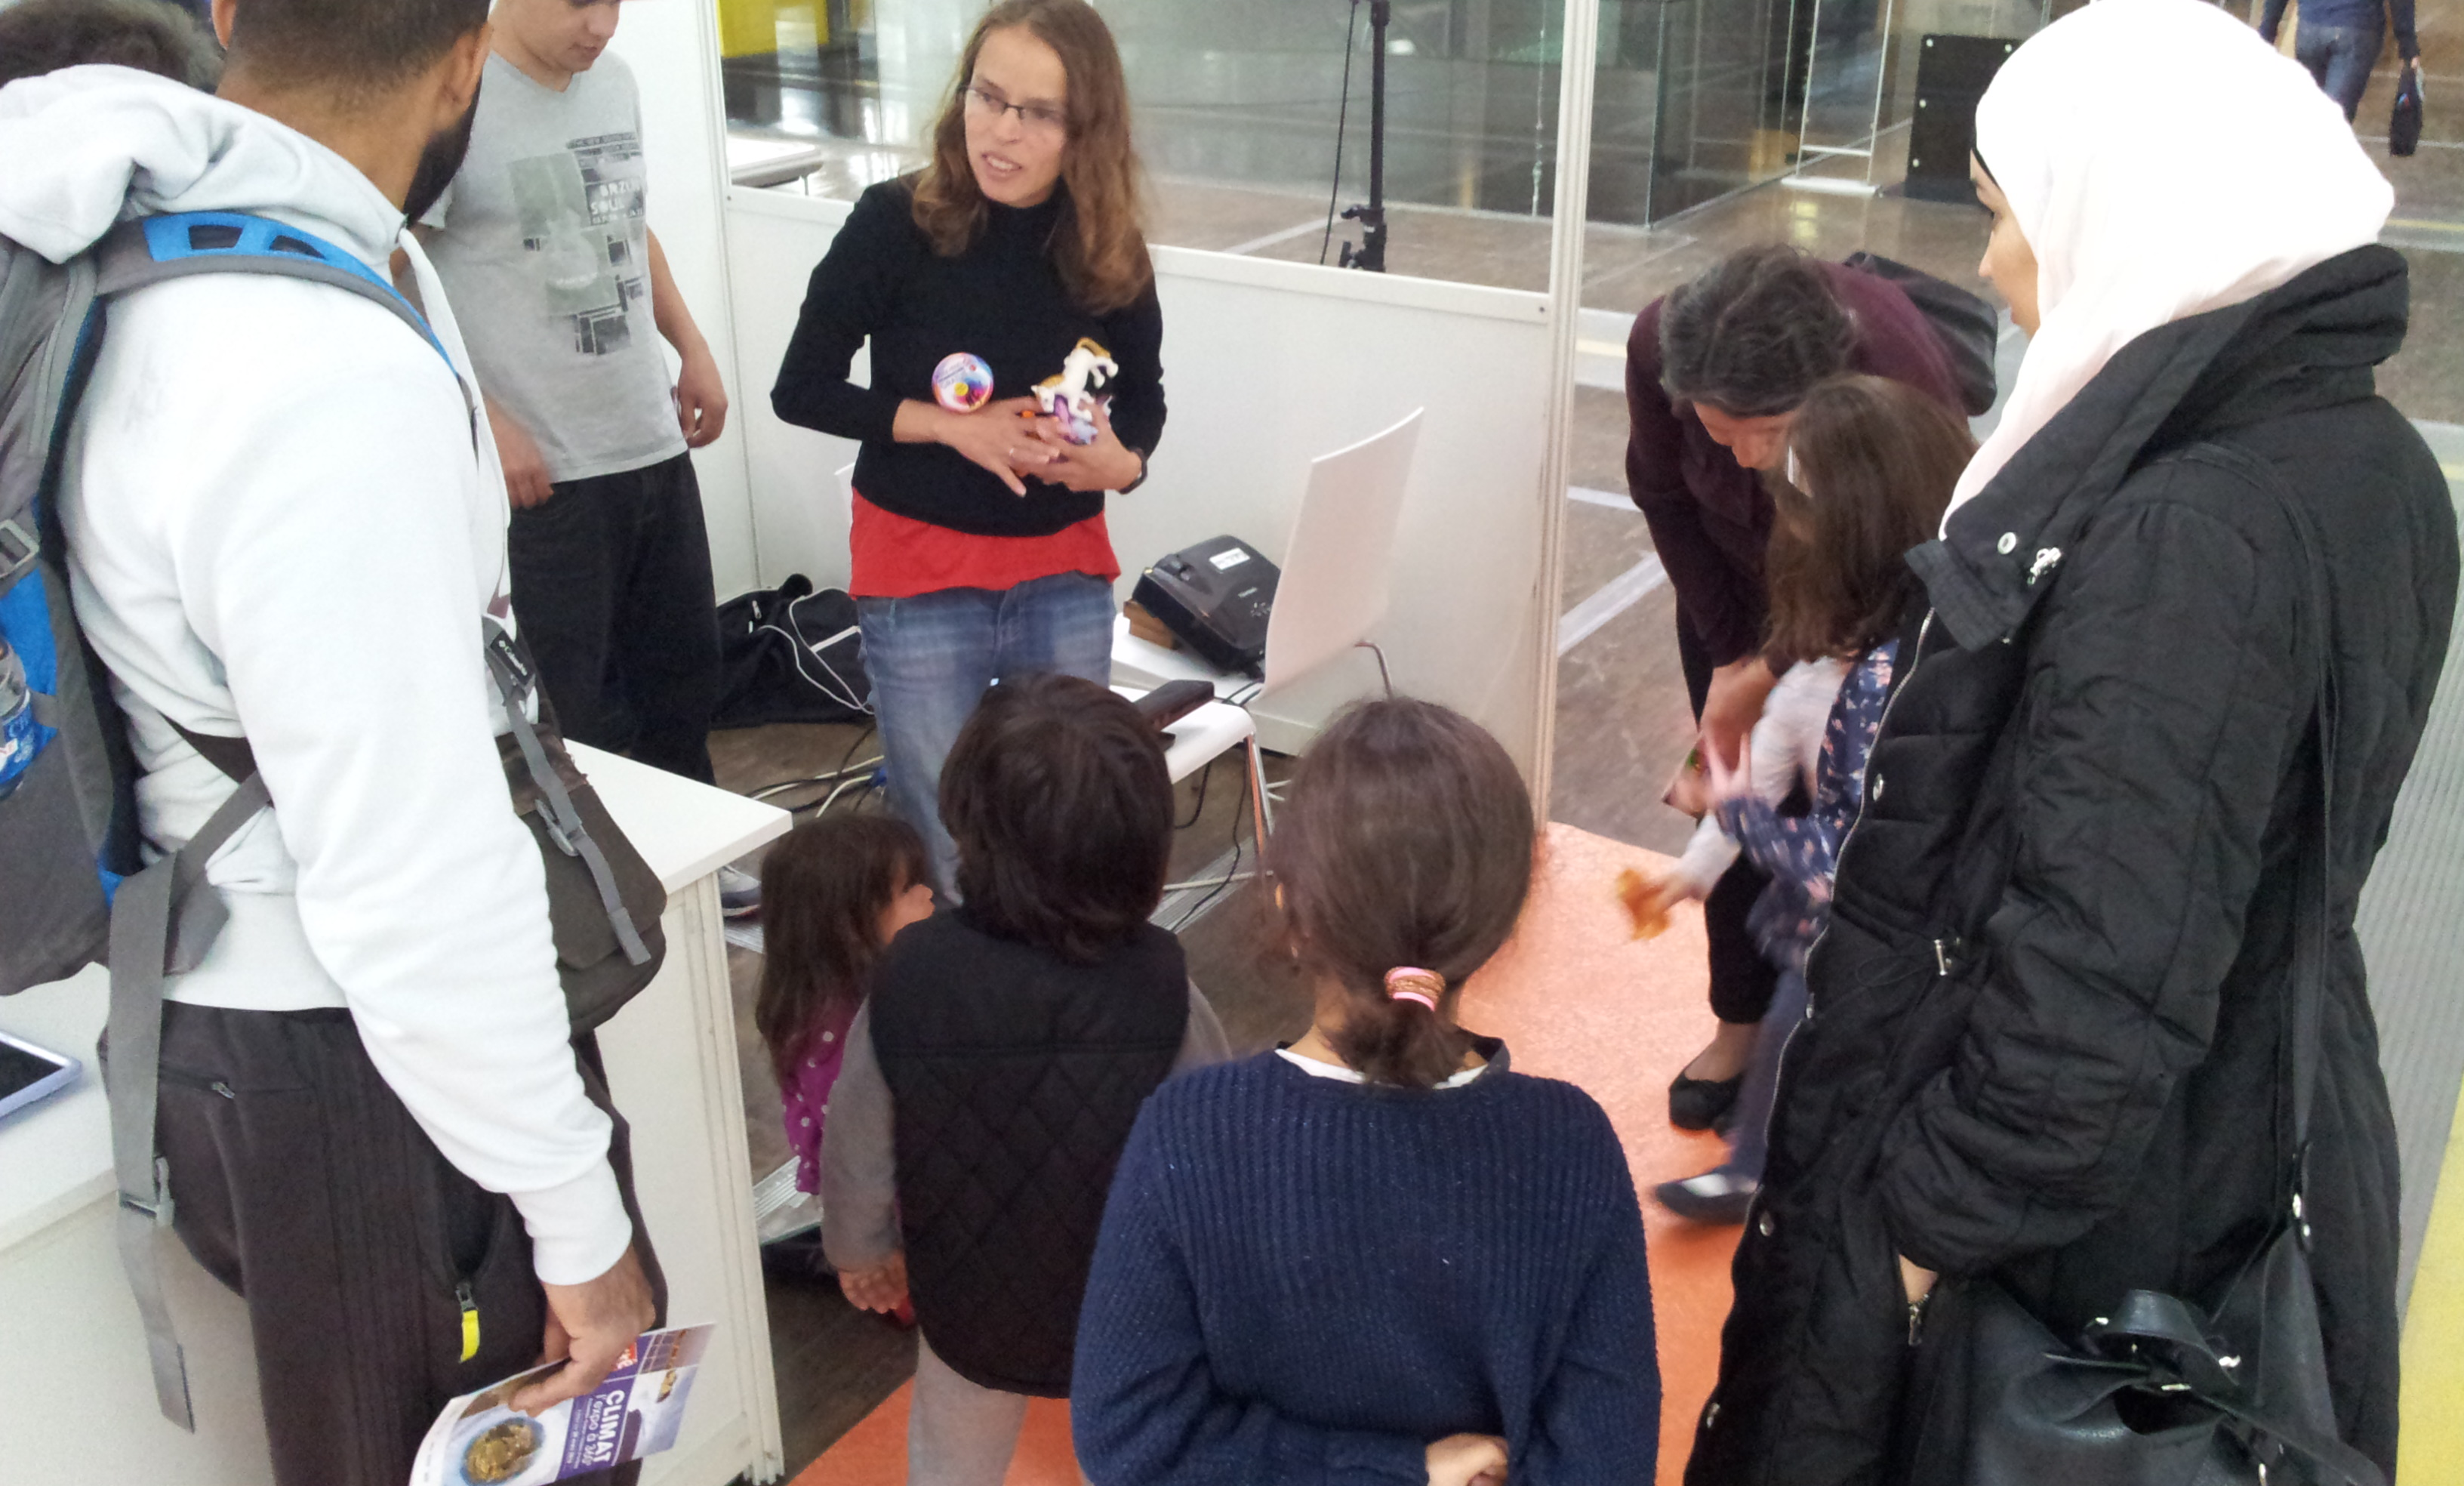
\includegraphics[width=\textwidth,height=0.2\textheight]{img/mirror1.jpg}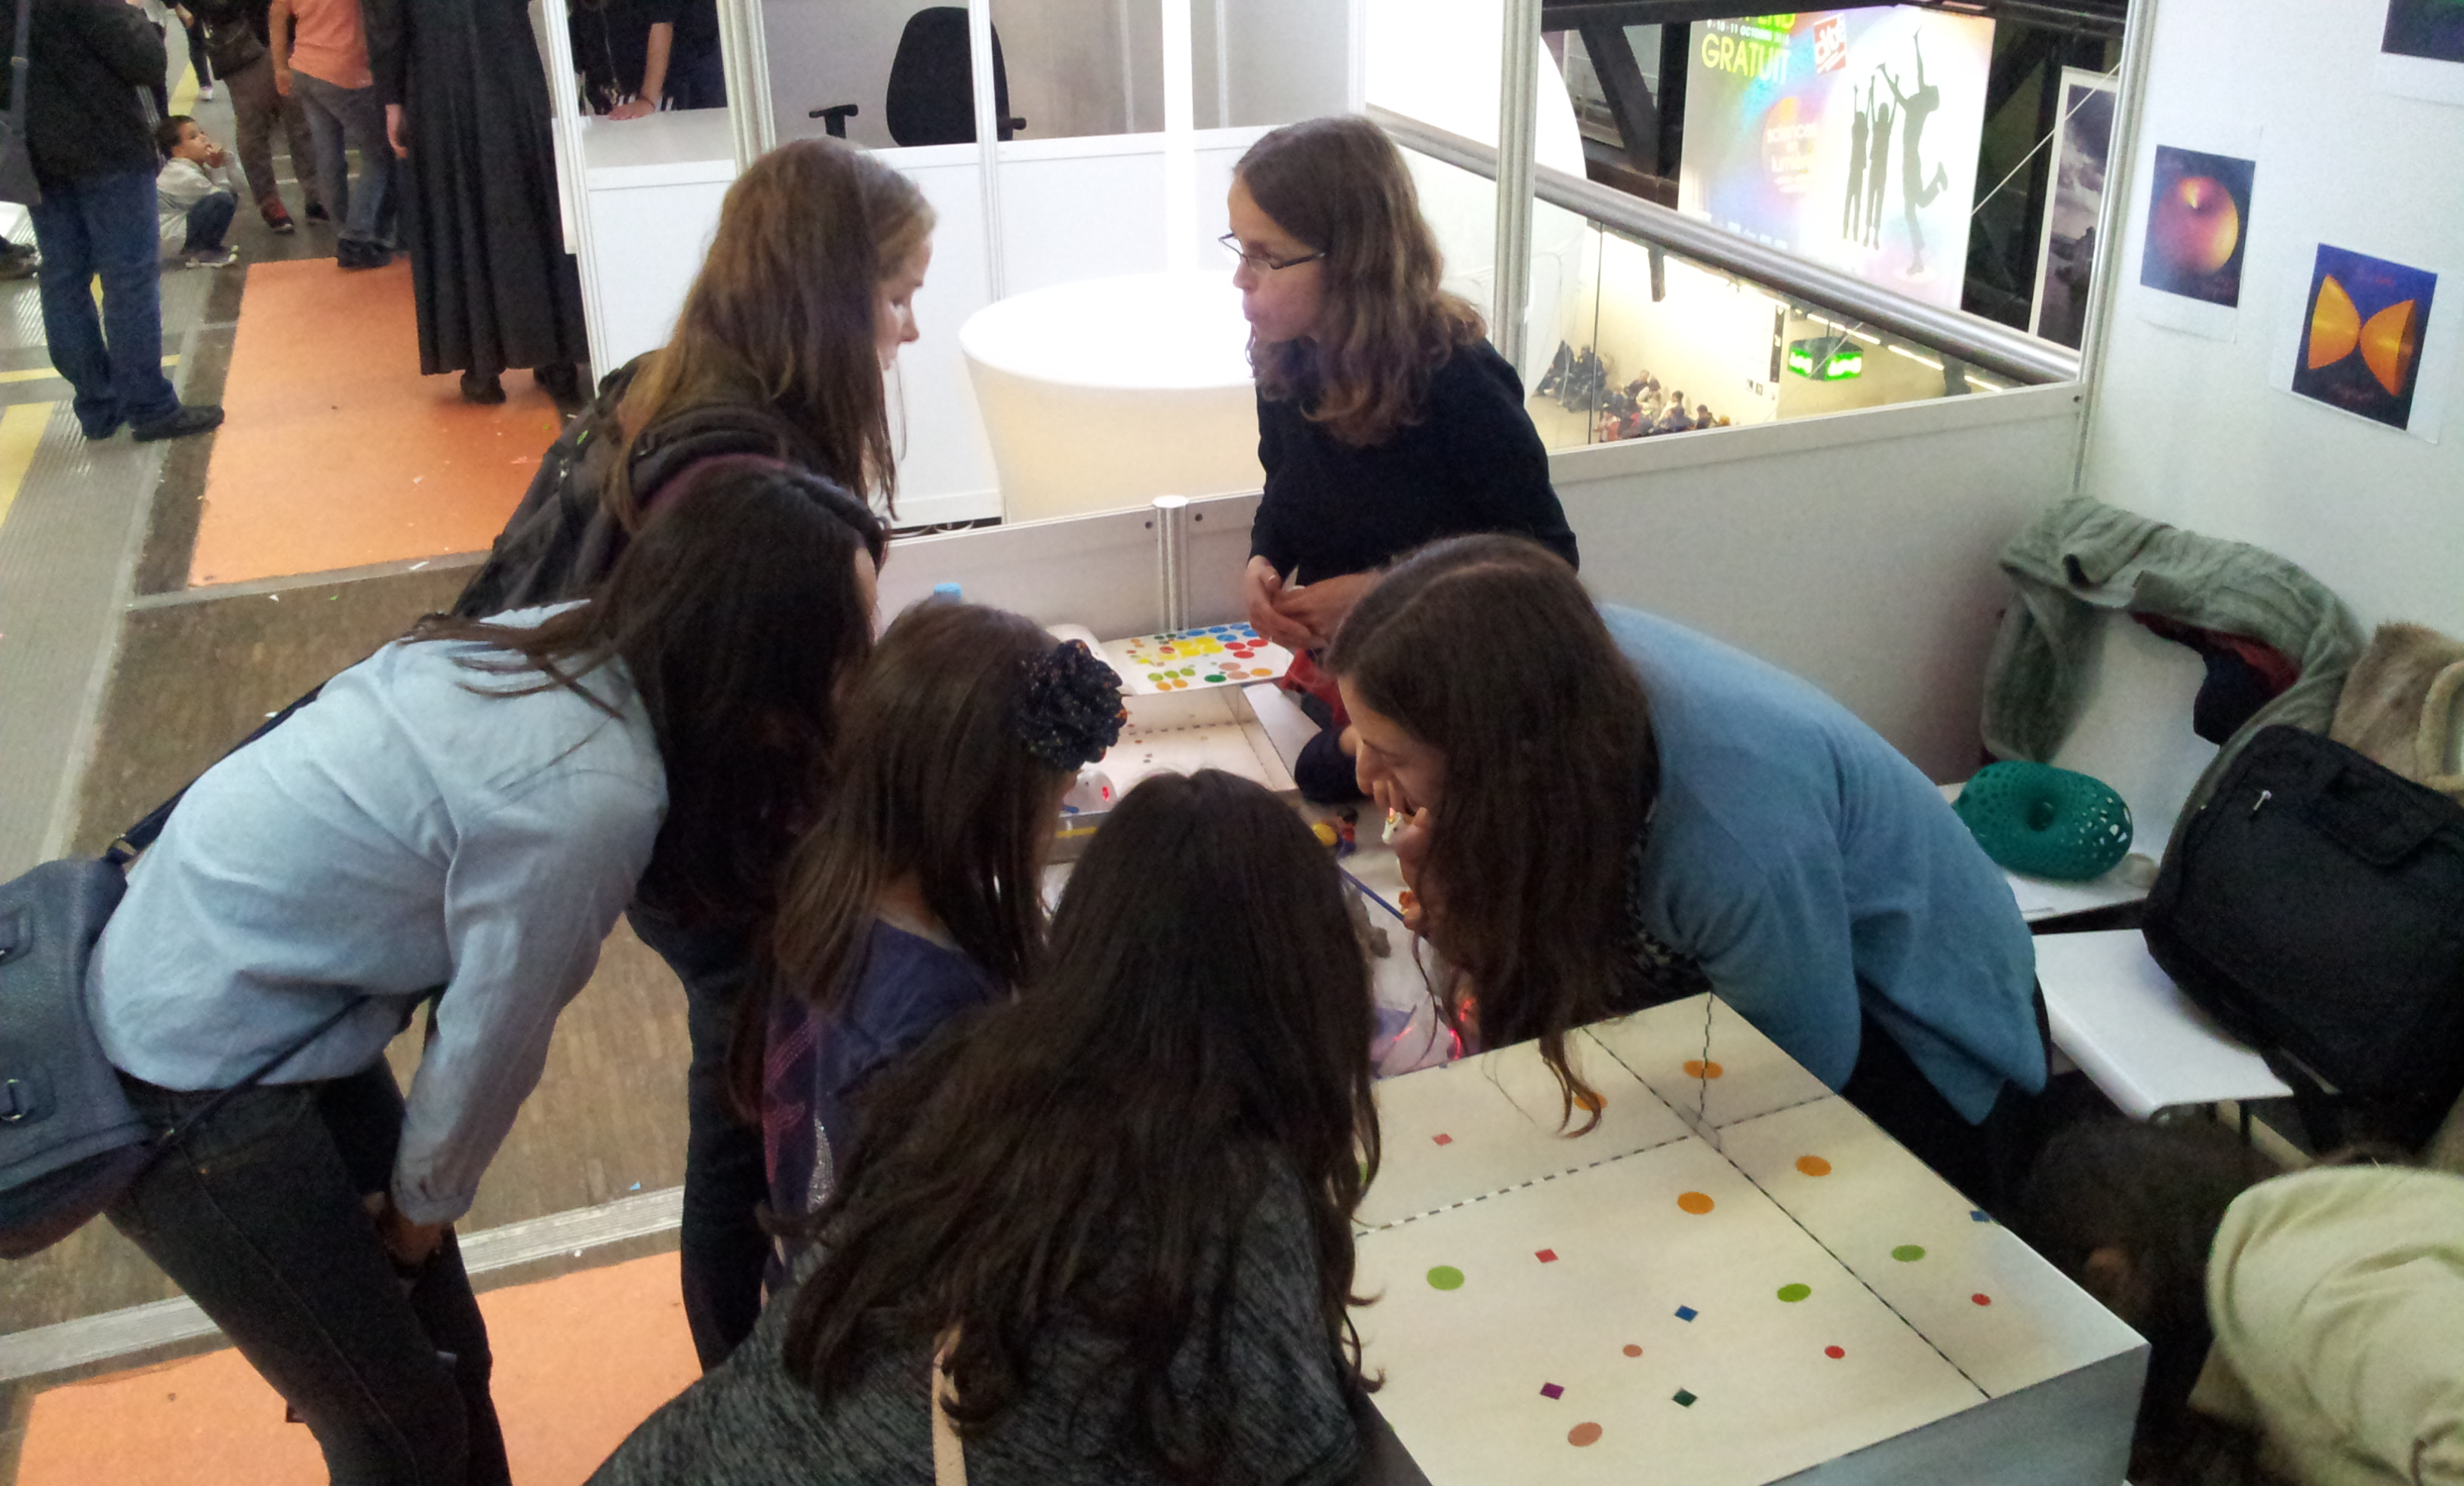
\includegraphics[width=\textwidth,height=0.25\textheight]{img/mirror2.jpg}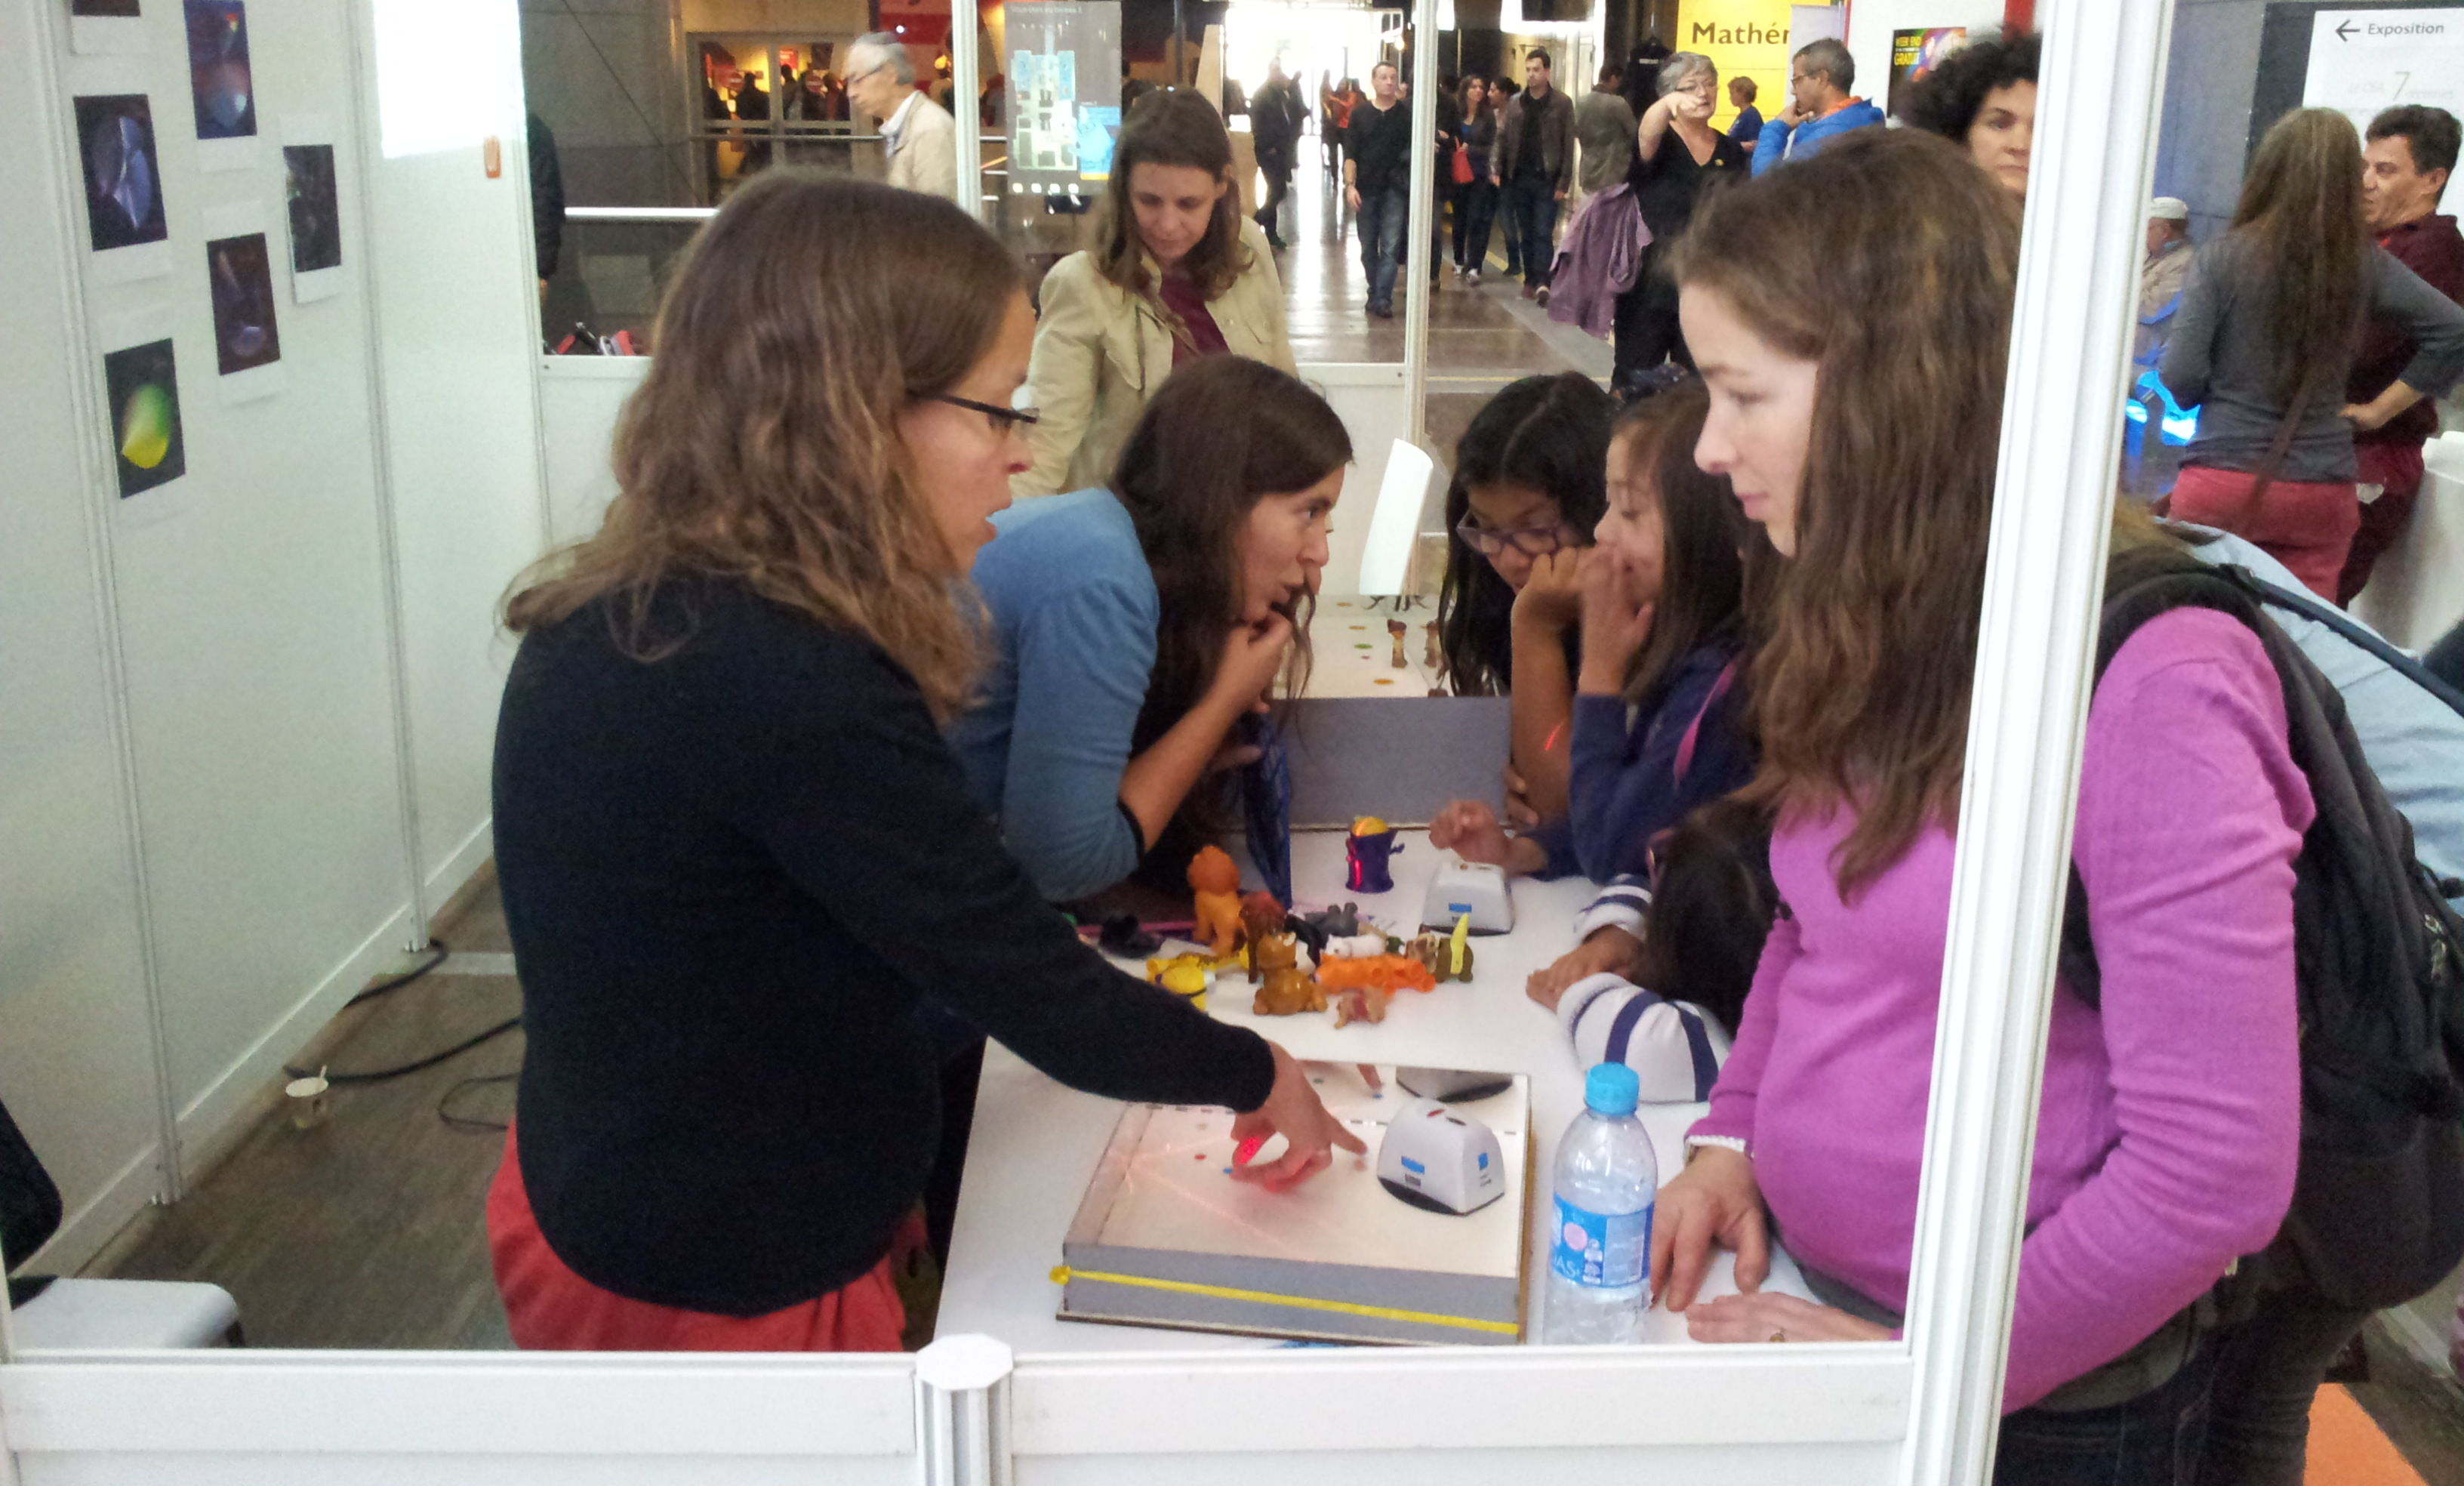
\includegraphics[width=\textwidth,height=0.2\textheight]{img/mirror3.jpg}

\par

\begin{itemize}
\tightlist
\item
  représentation interactive d'un théorème récent sur les billards
\item
  collaboration avec Samuel Lelièvre
\item
  financement:\\
  La Diagonale Paris-Saclay, Fondation Blaise Pascal
\end{itemize}
\end{block}
\end{frame}

\begin{frame}{Questions ?}
\protect\hypertarget{questions}{}
\begin{longtable}[]{@{}lll@{}}
\toprule
\endhead
\begin{minipage}[t]{0.32\columnwidth}\raggedright
parcours mixte math-info\strut
\end{minipage} & \begin{minipage}[t]{0.29\columnwidth}\raggedright
vrai souci de l'accessibilité\strut
\end{minipage} & \begin{minipage}[t]{0.30\columnwidth}\raggedright
fan de logiciels libres\strut
\end{minipage}\tabularnewline
\begin{minipage}[t]{0.32\columnwidth}\raggedright
\strut
\end{minipage} & \begin{minipage}[t]{0.29\columnwidth}\raggedright
\strut
\end{minipage} & \begin{minipage}[t]{0.30\columnwidth}\raggedright
\strut
\end{minipage}\tabularnewline
\begin{minipage}[t]{0.32\columnwidth}\raggedright
intérêt en médiation scientifique\strut
\end{minipage} & \begin{minipage}[t]{0.29\columnwidth}\raggedright
grand respect pour les étudiants\strut
\end{minipage} & \begin{minipage}[t]{0.30\columnwidth}\raggedright
continuité et ouverture dans la recherche\strut
\end{minipage}\tabularnewline
\begin{minipage}[t]{0.32\columnwidth}\raggedright
\strut
\end{minipage} & \begin{minipage}[t]{0.29\columnwidth}\raggedright
\strut
\end{minipage} & \begin{minipage}[t]{0.30\columnwidth}\raggedright
\strut
\end{minipage}\tabularnewline
\begin{minipage}[t]{0.32\columnwidth}\raggedright
facilités de contact\strut
\end{minipage} & \begin{minipage}[t]{0.29\columnwidth}\raggedright
fibre «maker»\strut
\end{minipage} & \begin{minipage}[t]{0.30\columnwidth}\raggedright
compétences techniques\strut
\end{minipage}\tabularnewline
\bottomrule
\end{longtable}

J'ai à cœur de m'intégrer dans la recherche chez Gamma3\\
et dans l'enseignement à l'UTT.

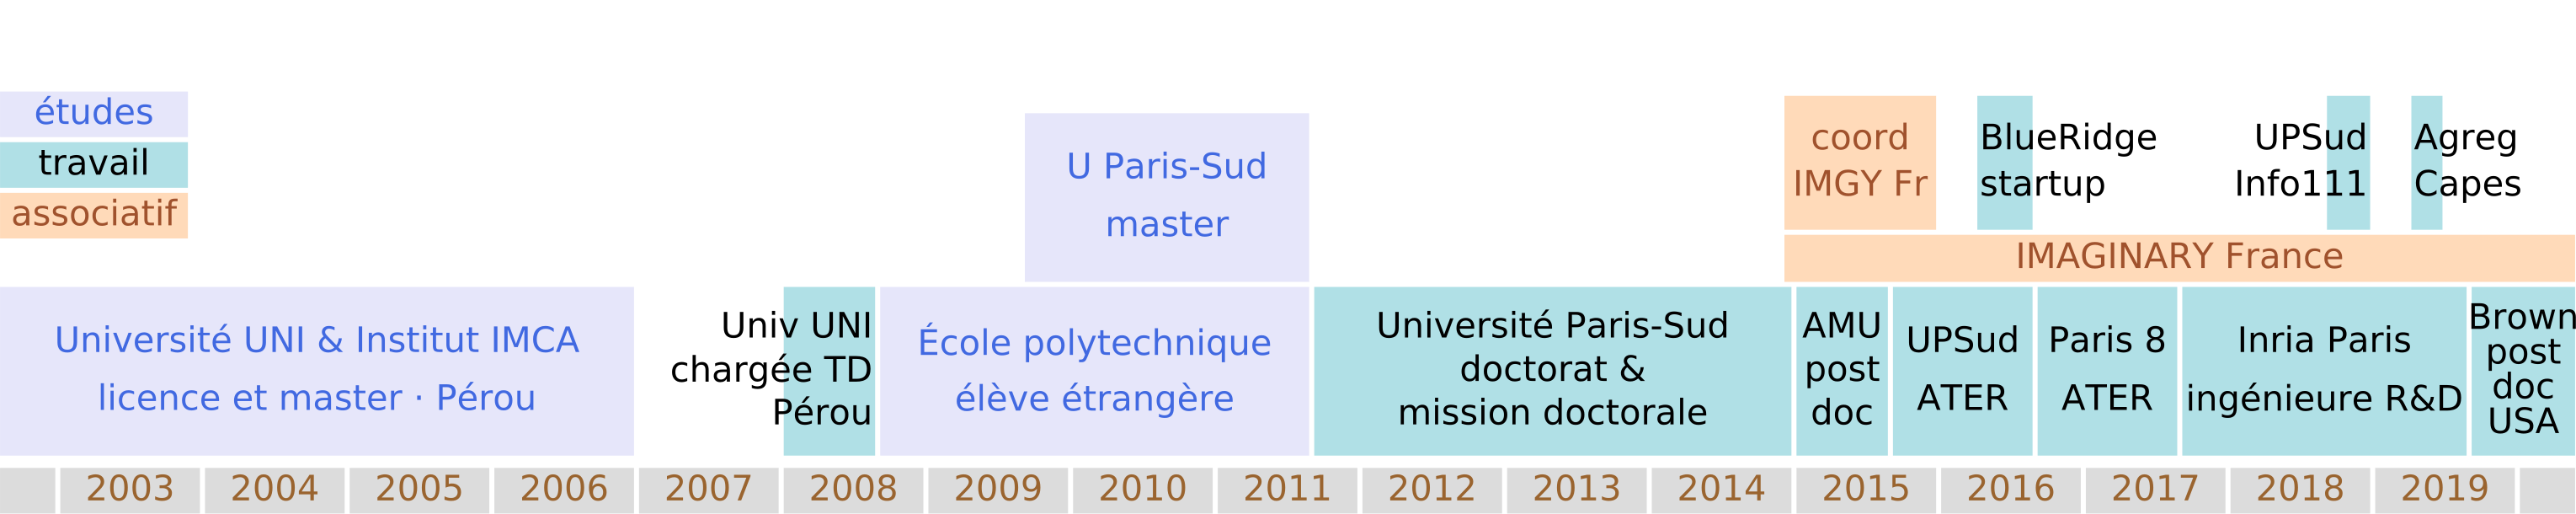
\includegraphics[width=1\textwidth,height=\textheight]{img/alba-timeline.png}
\end{frame}

\end{document}
